% Options for packages loaded elsewhere
\PassOptionsToPackage{unicode}{hyperref}
\PassOptionsToPackage{hyphens}{url}
\PassOptionsToPackage{dvipsnames,svgnames,x11names}{xcolor}
%
\documentclass[
  a4paper,
  noprof,
  12pt,
  notoc,
  nosols,
  nobib]{mnye}

\usepackage{amsmath,amssymb}
\usepackage{iftex}
\ifPDFTeX
  \usepackage[T1]{fontenc}
  \usepackage[utf8]{inputenc}
  \usepackage{textcomp} % provide euro and other symbols
\else % if luatex or xetex
  \usepackage{unicode-math}
  \defaultfontfeatures{Scale=MatchLowercase}
  \defaultfontfeatures[\rmfamily]{Ligatures=TeX,Scale=1}
\fi
\usepackage{lmodern}
\ifPDFTeX\else  
    % xetex/luatex font selection
\fi
% Use upquote if available, for straight quotes in verbatim environments
\IfFileExists{upquote.sty}{\usepackage{upquote}}{}
\IfFileExists{microtype.sty}{% use microtype if available
  \usepackage[]{microtype}
  \UseMicrotypeSet[protrusion]{basicmath} % disable protrusion for tt fonts
}{}
\makeatletter
\@ifundefined{KOMAClassName}{% if non-KOMA class
  \IfFileExists{parskip.sty}{%
    \usepackage{parskip}
  }{% else
    \setlength{\parindent}{0pt}
    \setlength{\parskip}{6pt plus 2pt minus 1pt}}
}{% if KOMA class
  \KOMAoptions{parskip=half}}
\makeatother
\usepackage{xcolor}
\setlength{\emergencystretch}{3em} % prevent overfull lines
\setcounter{secnumdepth}{5}
% Make \paragraph and \subparagraph free-standing
\ifx\paragraph\undefined\else
  \let\oldparagraph\paragraph
  \renewcommand{\paragraph}[1]{\oldparagraph{#1}\mbox{}}
\fi
\ifx\subparagraph\undefined\else
  \let\oldsubparagraph\subparagraph
  \renewcommand{\subparagraph}[1]{\oldsubparagraph{#1}\mbox{}}
\fi

\usepackage{color}
\usepackage{fancyvrb}
\newcommand{\VerbBar}{|}
\newcommand{\VERB}{\Verb[commandchars=\\\{\}]}
\DefineVerbatimEnvironment{Highlighting}{Verbatim}{commandchars=\\\{\}}
% Add ',fontsize=\small' for more characters per line
\usepackage{framed}
\definecolor{shadecolor}{RGB}{241,243,245}
\newenvironment{Shaded}{\begin{snugshade}}{\end{snugshade}}
\newcommand{\AlertTok}[1]{\textcolor[rgb]{0.68,0.00,0.00}{#1}}
\newcommand{\AnnotationTok}[1]{\textcolor[rgb]{0.37,0.37,0.37}{#1}}
\newcommand{\AttributeTok}[1]{\textcolor[rgb]{0.40,0.45,0.13}{#1}}
\newcommand{\BaseNTok}[1]{\textcolor[rgb]{0.68,0.00,0.00}{#1}}
\newcommand{\BuiltInTok}[1]{\textcolor[rgb]{0.00,0.23,0.31}{#1}}
\newcommand{\CharTok}[1]{\textcolor[rgb]{0.13,0.47,0.30}{#1}}
\newcommand{\CommentTok}[1]{\textcolor[rgb]{0.37,0.37,0.37}{#1}}
\newcommand{\CommentVarTok}[1]{\textcolor[rgb]{0.37,0.37,0.37}{\textit{#1}}}
\newcommand{\ConstantTok}[1]{\textcolor[rgb]{0.56,0.35,0.01}{#1}}
\newcommand{\ControlFlowTok}[1]{\textcolor[rgb]{0.00,0.23,0.31}{#1}}
\newcommand{\DataTypeTok}[1]{\textcolor[rgb]{0.68,0.00,0.00}{#1}}
\newcommand{\DecValTok}[1]{\textcolor[rgb]{0.68,0.00,0.00}{#1}}
\newcommand{\DocumentationTok}[1]{\textcolor[rgb]{0.37,0.37,0.37}{\textit{#1}}}
\newcommand{\ErrorTok}[1]{\textcolor[rgb]{0.68,0.00,0.00}{#1}}
\newcommand{\ExtensionTok}[1]{\textcolor[rgb]{0.00,0.23,0.31}{#1}}
\newcommand{\FloatTok}[1]{\textcolor[rgb]{0.68,0.00,0.00}{#1}}
\newcommand{\FunctionTok}[1]{\textcolor[rgb]{0.28,0.35,0.67}{#1}}
\newcommand{\ImportTok}[1]{\textcolor[rgb]{0.00,0.46,0.62}{#1}}
\newcommand{\InformationTok}[1]{\textcolor[rgb]{0.37,0.37,0.37}{#1}}
\newcommand{\KeywordTok}[1]{\textcolor[rgb]{0.00,0.23,0.31}{#1}}
\newcommand{\NormalTok}[1]{\textcolor[rgb]{0.00,0.23,0.31}{#1}}
\newcommand{\OperatorTok}[1]{\textcolor[rgb]{0.37,0.37,0.37}{#1}}
\newcommand{\OtherTok}[1]{\textcolor[rgb]{0.00,0.23,0.31}{#1}}
\newcommand{\PreprocessorTok}[1]{\textcolor[rgb]{0.68,0.00,0.00}{#1}}
\newcommand{\RegionMarkerTok}[1]{\textcolor[rgb]{0.00,0.23,0.31}{#1}}
\newcommand{\SpecialCharTok}[1]{\textcolor[rgb]{0.37,0.37,0.37}{#1}}
\newcommand{\SpecialStringTok}[1]{\textcolor[rgb]{0.13,0.47,0.30}{#1}}
\newcommand{\StringTok}[1]{\textcolor[rgb]{0.13,0.47,0.30}{#1}}
\newcommand{\VariableTok}[1]{\textcolor[rgb]{0.07,0.07,0.07}{#1}}
\newcommand{\VerbatimStringTok}[1]{\textcolor[rgb]{0.13,0.47,0.30}{#1}}
\newcommand{\WarningTok}[1]{\textcolor[rgb]{0.37,0.37,0.37}{\textit{#1}}}

\providecommand{\tightlist}{%
  \setlength{\itemsep}{0pt}\setlength{\parskip}{0pt}}\usepackage{longtable,booktabs,array}
\usepackage{calc} % for calculating minipage widths
% Correct order of tables after \paragraph or \subparagraph
\usepackage{etoolbox}
\makeatletter
\patchcmd\longtable{\par}{\if@noskipsec\mbox{}\fi\par}{}{}
\makeatother
% Allow footnotes in longtable head/foot
\IfFileExists{footnotehyper.sty}{\usepackage{footnotehyper}}{\usepackage{footnote}}
\makesavenoteenv{longtable}
\usepackage{graphicx}
\makeatletter
\def\maxwidth{\ifdim\Gin@nat@width>\linewidth\linewidth\else\Gin@nat@width\fi}
\def\maxheight{\ifdim\Gin@nat@height>\textheight\textheight\else\Gin@nat@height\fi}
\makeatother
% Scale images if necessary, so that they will not overflow the page
% margins by default, and it is still possible to overwrite the defaults
% using explicit options in \includegraphics[width, height, ...]{}
\setkeys{Gin}{width=\maxwidth,height=\maxheight,keepaspectratio}
% Set default figure placement to htbp
\makeatletter
\def\fps@figure{htbp}
\makeatother

\usepackage{ehyperref}


\AtBeginDocument{
    \ifcsname c@theorem\endcsname % el contador theorem no está definido hasta que no se usa :::{#thm-label}
        \counterwithout{theorem}{section}
    \fi
    % \counterwithout{exercise}{section}
}

\AtBeginDocument{

    % Los entornos de teoremas que crea Quarto no están definidos hasta que no se usan.
    % Por ejemplo, exercise no está definido hasta que no se usa :::{#exr-label}

    % definition
    \ifcsname enddefinition\endcsname 
    \renewenvironment{definition}[1][]{
        \if\relax\detokenize{#1}\relax
            \dfn
        \else
            \dfn[note={#1}]
        \fi
    }{\enddfn}
    \fi

    % theorem
    \ifcsname endtheorem\endcsname 
    \renewenvironment{theorem}[1][]{%
        \if\relax\detokenize{#1}\relax%
            \thm%
        \else%
            \thm[note={#1}]%
        \fi%
        \unskip\unskip\ignorespaces
    }{\endthm}
    \fi   
    
    

    % example
    \ifcsname endexample\endcsname %
        \renewenvironment{example}[1][]{
            \if\relax\detokenize{#1}\relax
                \exmp
            \else
                \exmp[note={#1}]
            \fi
        }{\endex}
    \fi

    % exercise
    \ifcsname endexercise\endcsname %
        \renewenvironment{exercise}[1][]{
            \if\relax\detokenize{#1}\relax
                \ex
            \else
                \ex[note={#1}]
            \fi
        }{\endex}
    \fi

    % solution
    \ifcsname endsolution\endcsname 
        \renewenvironment{solution}{
                \sol
        }{\endsol}
    \fi
}
\graphicspath{{docs/}{./}}
\usepackage{fvextra}
\DefineVerbatimEnvironment{Highlighting}{Verbatim}{breaklines,commandchars=\\\{\}}
\usepackage{multido}
\tikzexternaldisable
\makeatletter
\@ifpackageloaded{tcolorbox}{}{\usepackage[skins,breakable]{tcolorbox}}
\@ifpackageloaded{fontawesome5}{}{\usepackage{fontawesome5}}
\definecolor{quarto-callout-color}{HTML}{909090}
\definecolor{quarto-callout-note-color}{HTML}{0758E5}
\definecolor{quarto-callout-important-color}{HTML}{CC1914}
\definecolor{quarto-callout-warning-color}{HTML}{EB9113}
\definecolor{quarto-callout-tip-color}{HTML}{00A047}
\definecolor{quarto-callout-caution-color}{HTML}{FC5300}
\definecolor{quarto-callout-color-frame}{HTML}{acacac}
\definecolor{quarto-callout-note-color-frame}{HTML}{4582ec}
\definecolor{quarto-callout-important-color-frame}{HTML}{d9534f}
\definecolor{quarto-callout-warning-color-frame}{HTML}{f0ad4e}
\definecolor{quarto-callout-tip-color-frame}{HTML}{02b875}
\definecolor{quarto-callout-caution-color-frame}{HTML}{fd7e14}
\makeatother
\makeatletter
\@ifpackageloaded{bookmark}{}{\usepackage{bookmark}}
\makeatother
\makeatletter
\@ifpackageloaded{caption}{}{\usepackage{caption}}
\AtBeginDocument{%
\ifdefined\contentsname
  \renewcommand*\contentsname{Tabla de contenidos}
\else
  \newcommand\contentsname{Tabla de contenidos}
\fi
\ifdefined\listfigurename
  \renewcommand*\listfigurename{Listado de Figuras}
\else
  \newcommand\listfigurename{Listado de Figuras}
\fi
\ifdefined\listtablename
  \renewcommand*\listtablename{Listado de Tablas}
\else
  \newcommand\listtablename{Listado de Tablas}
\fi
\ifdefined\figurename
  \renewcommand*\figurename{Figura}
\else
  \newcommand\figurename{Figura}
\fi
\ifdefined\tablename
  \renewcommand*\tablename{Tabla}
\else
  \newcommand\tablename{Tabla}
\fi
}
\@ifpackageloaded{float}{}{\usepackage{float}}
\floatstyle{ruled}
\@ifundefined{c@chapter}{\newfloat{codelisting}{h}{lop}}{\newfloat{codelisting}{h}{lop}[chapter]}
\floatname{codelisting}{Listado}
\newcommand*\listoflistings{\listof{codelisting}{Listado de Listados}}
\usepackage{amsthm}
\theoremstyle{definition}
\newtheorem{exercise}{Ejercicio}[section]
\theoremstyle{remark}
\AtBeginDocument{\renewcommand*{\proofname}{Prueba}}
\newtheorem*{remark}{Observación}
\newtheorem*{solution}{Solución}
\newtheorem{refremark}{Observación}[section]
\newtheorem{refsolution}{Solución}[section]
\makeatother
\makeatletter
\makeatother
\makeatletter
\@ifpackageloaded{caption}{}{\usepackage{caption}}
\@ifpackageloaded{subcaption}{}{\usepackage{subcaption}}
\makeatother
\ifLuaTeX
\usepackage[bidi=basic]{babel}
\else
\usepackage[bidi=default]{babel}
\fi
\babelprovide[main,import]{spanish}
% get rid of language-specific shorthands (see #6817):
\let\LanguageShortHands\languageshorthands
\def\languageshorthands#1{}
\ifLuaTeX
  \usepackage{selnolig}  % disable illegal ligatures
\fi
\usepackage[backend=biber]{biblatex}
\addbibresource{references.bib}
\nocite{reback2020pandas, mckinney-proc-scipy-2010, Waskom2021}
\usepackage{bookmark}

\IfFileExists{xurl.sty}{\usepackage{xurl}}{} % add URL line breaks if available
\urlstyle{same} % disable monospaced font for URLs
\hypersetup{
  pdftitle={Exploración y visualización de datos con Python},
  pdfauthor={Eva María Mazcuñán Navarro},
  pdflang={es},
  colorlinks=true,
  linkcolor={elinkcolor},
  filecolor={Maroon},
  citecolor={ecitecolor},
  urlcolor={eurlcolor},
  pdfcreator={LaTeX via pandoc}}

\title{Exploración y visualización de datos con Python}
\term{2023-2024}
\degree{Grado en Ingeniería Informática / Mecánica}
\author{Eva María Mazcuñán Navarro}
\date{}

\begin{document}
\maketitle

\renewcommand*\contentsname{Contenidos}
{
\hypersetup{linkcolor=elinkcolor}
\pagenumbering{roman}%
\pagestyle{plain}%
\setcounter{tocdepth}{2}
\tableofcontents
\cleardoublepage{
\pagenumbering{arabic}%
\pagestyle{main}}
}
\bookmarksetup{startatroot}

\addcontentsline{toc}{section}{Inicio}


\bookmarksetup{startatroot}

\section*{Introducción}\label{sec-intro}
\addcontentsline{toc}{section}{Introducción}


En esta práctica aprenderás las técnicas básicas para explorar y
visualizar un conjunto de datos con Python.

\subsection*{Los pingüinos del archipiélago
Palmer}\label{los-pinguxfcinos-del-archipiuxe9lago-palmer}
\addcontentsline{toc}{subsection}{Los pingüinos del archipiélago Palmer}


Presentaremos las diferentes técnicas a través de ejemplos trabajando
con un conjunto de datos relativos a diferentes características de tres
especies de pingüinos del archipiélago Palmer en la Antártida.

\begin{figure}[tbph]

{\centering 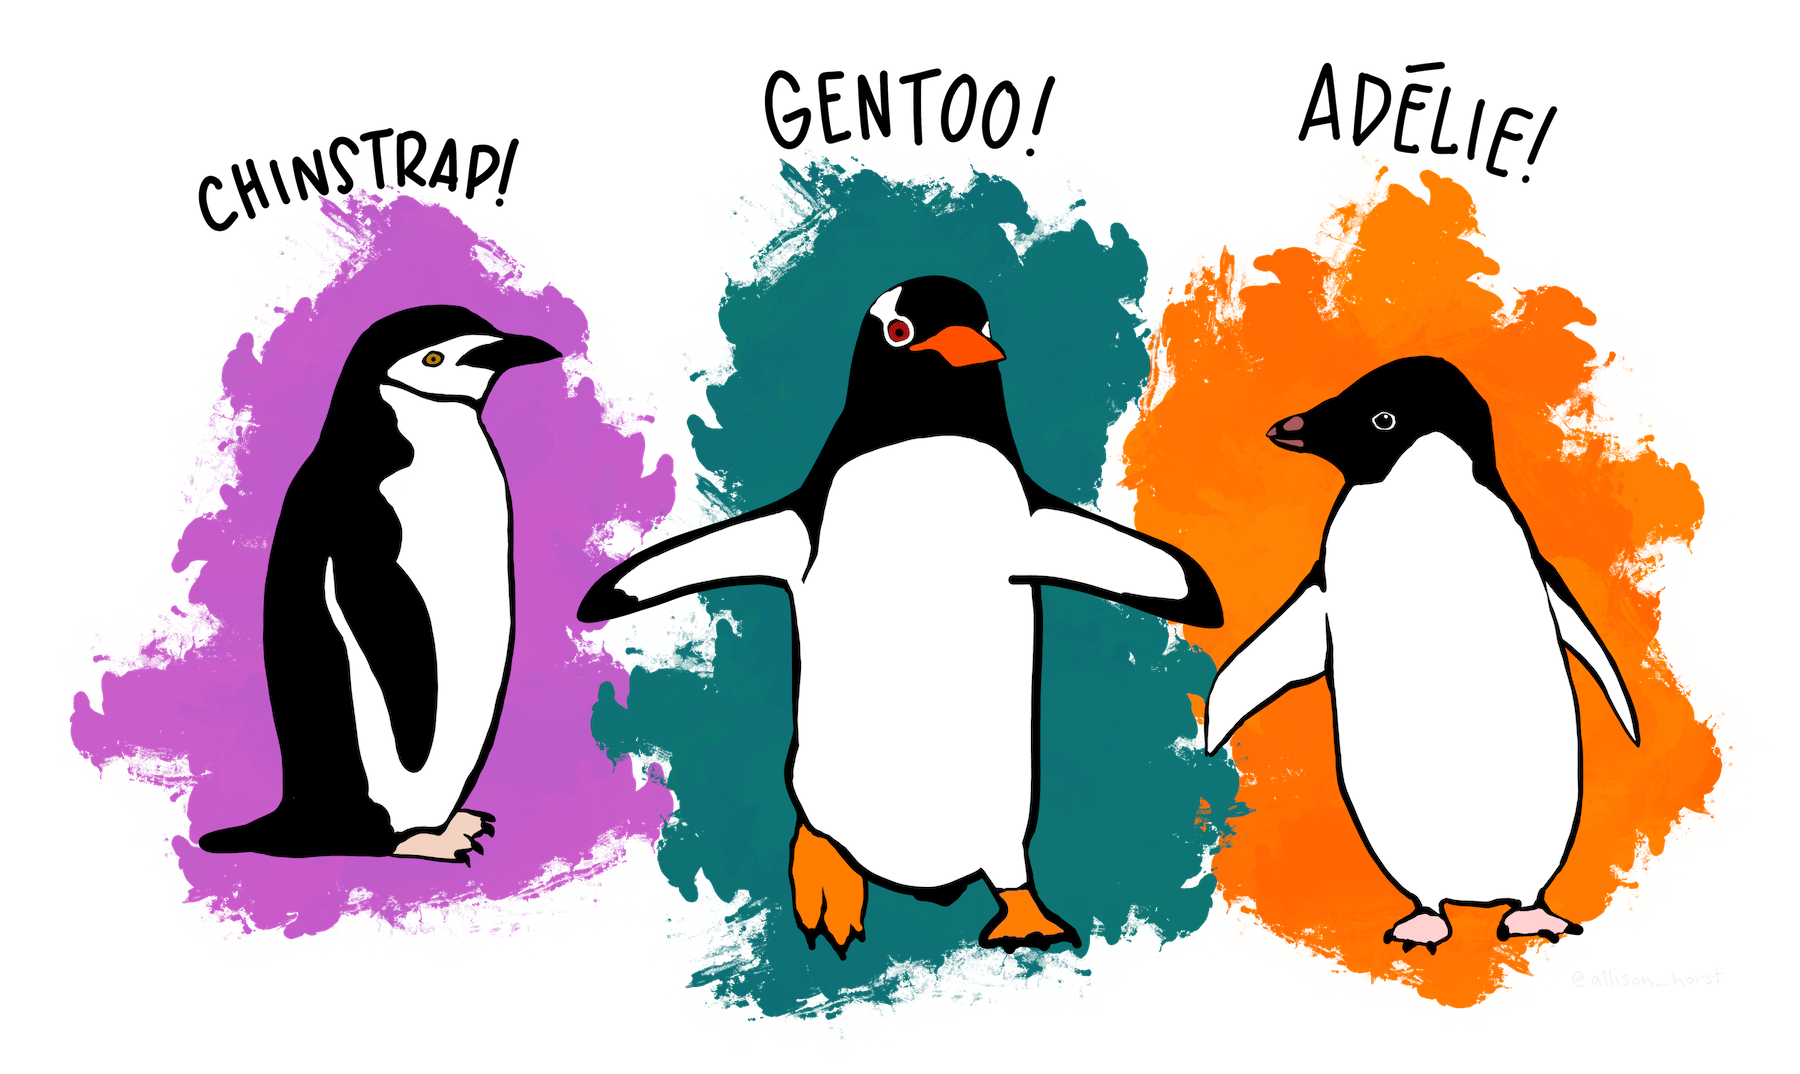
\includegraphics[width=0.8\textwidth,height=\textheight]{chapters/../img/penguins.png}

}

\caption{Ilustración de las tres especies de pingüinos del archipiélago
Palmer (Artista @allison\_horst)}

\end{figure}%

Los datos fueron originalmente publicados en \textcite{Gorman2014}. Este
conjunto de datos se hizo popular a partir de la creación del paquete
\href{https://github.com/allisonhorst/palmerpenguins}{palmerpenguins} de
\href{https://www.r-project.org/}{R}. Hoy en día los datos de los
pingüinos del archipiélago Palmer se usan de forma extendida para
ilustrar las técnicas de exploración y visualización de datos no solo en
R, sino en muchos otros lenguajes de programación para estadística y
ciencia de datos, como Python. Nosotros accederemos a los datos a través
de
\href{https://github.com/mwaskom/seaborn-data/blob/master/penguins.csv}{este
enlace}, que proporciona los datos en formato CSV (\emph{comma separated
values}).

\subsection*{Objetivos}\label{objetivos}
\addcontentsline{toc}{subsection}{Objetivos}


Aprenderás en concreto a calcular las medidas descriptivas más
representativas de las características de interés y a crear diferentes
tipos de gráficos o visualizaciones.

\bookmarksetup{startatroot}

\section{Librerías}\label{libreruxedas}

Lo primero que necesitamos hacer es importar las librerías de Python que
usaremos a lo largo de práctica, que son \texttt{pandas} y
\texttt{seaborn}:

\begin{Shaded}
\begin{Highlighting}[]
\ImportTok{import}\NormalTok{ pandas }\ImportTok{as}\NormalTok{ pd}
\ImportTok{import}\NormalTok{ seaborn }\ImportTok{as}\NormalTok{ sns}
\end{Highlighting}
\end{Shaded}

\subsection{\texorpdfstring{\texttt{pandas}}{pandas}}\label{pandas}

\begin{center}

\includegraphics[width=\textwidth,height=4em]{chapters/../img/pandas.png}
\end{center}

\texttt{pandas} es una librería que permite leer datos almacenados en
estructuras similares a una tabla, como las hojas de cálculo o los
archivos CSV, y proporciona métodos para explorar y describir esos
datos.

Usando esta librería podremos calcular por ejemplo el peso medio de los
pingüinos de cada especie. Obtendremos esta tabla:

\begin{verbatim}
species
Adelie       3700.662252
Chinstrap    3733.088235
Gentoo       5076.016260
Name: body_mass_g, dtype: float64
\end{verbatim}

Puedes consultar la documentación oficial de \texttt{pandas}
\href{https://pandas.pydata.org/docs/index.html}{aquí}.

\subsection{\texorpdfstring{\texttt{seaborn}}{seaborn}}\label{seaborn}

\begin{center}

\includegraphics[width=\textwidth,height=3em]{chapters/../img/seaborn.png}
\end{center}

\texttt{seaborn} es una librería para visualización de datos. Permite
crear gráficos estadísticos muy informativos y visualmente atractivos
con pocas líneas de código. Y está diseñado para trabajar con las
estructuras de datos creadas con \texttt{pandas}.

Usaremos \texttt{seaborn} para realizar diferentes tipos de gráficos
como diagramas de barras, histogramas, diagramas de caja y bigotes etc.

Aprenderemos por ejemplo a crear el siguiente gráfico, con los diagramas
de caja y bigotes para el peso de los pingüinos de cada especie.

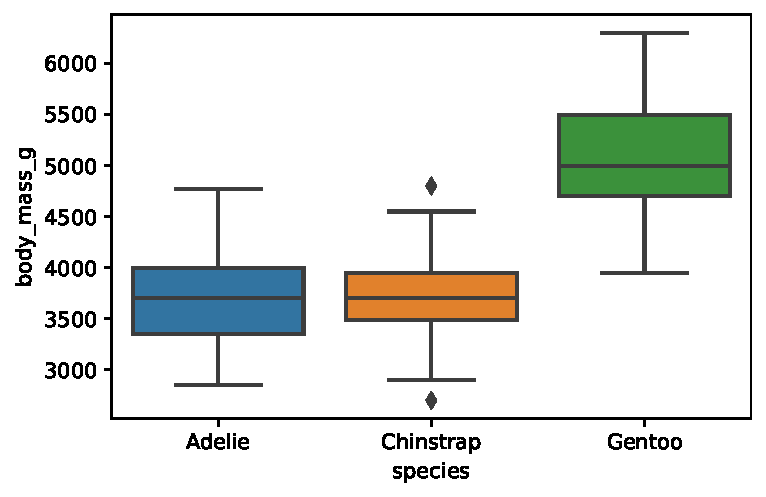
\includegraphics{chapters/libraries_files/figure-pdf/cell-5-output-1.pdf}

Puedes consultar la documentación oficial de \texttt{seaborn}
\href{https://seaborn.pydata.org/index.html}{aquí}.

\bookmarksetup{startatroot}

\section{Datos}\label{datos}

En esta sección importarás los datos sobre los pingüinos del
archipiélago Palmer presentados en la introducción y conocerás la
información que contienen.

\subsection{Importar los datos}\label{importar-los-datos}

Como se indicó en la introducción, los datos con los que vamos a
trabajar están disponibles en la web en un fichero de formato
\texttt{CSV}.

Ejecuta las instrucciones a continuación para importar el archivo usando
la función \texttt{read\_csv()} y guardar el resultado en una variable
de nombre \texttt{penguins}:

\begin{Shaded}
\begin{Highlighting}[]
\NormalTok{url }\OperatorTok{=} \StringTok{"https://raw.githubusercontent.com/mwaskom/seaborn{-}data/master/penguins.csv"}
\NormalTok{penguins }\OperatorTok{=}\NormalTok{ pd.read\_csv(url)}
\end{Highlighting}
\end{Shaded}

El objeto \texttt{penguins} que acabas de crear es una \textbf{hoja de
datos}, representada en \texttt{pandas} con la clase \texttt{DataFrame}.

\begin{Shaded}
\begin{Highlighting}[]
\BuiltInTok{type}\NormalTok{(penguins)}
\end{Highlighting}
\end{Shaded}

\begin{verbatim}
pandas.core.frame.DataFrame
\end{verbatim}

En los siguientes apartados aprenderás a realizar una exploración
inicial de la hoja de datos \texttt{penguins} que acabas de crear para
conocer su estructura y la información que contiene.

\subsection{Dimensiones}\label{dimensiones}

Una hoja de datos es una estructura matricial o tabular que contiene
datos organizados por filas y columnas.

Para saber las dimensiones de nuestra hoja de datos \texttt{penguins}
consulta su propiedad \texttt{shape}:

\begin{Shaded}
\begin{Highlighting}[]
\NormalTok{penguins.shape}
\end{Highlighting}
\end{Shaded}

\begin{verbatim}
(344, 7)
\end{verbatim}

Vemos que nuestra hoja de datos tiene \texttt{344} filas y \texttt{7}
columnas.

\subsection{Primeras y últimas filas}\label{sec-head-tail}

Con las siguientes instrucciones puedes visualizar las cinco primeras y
últimas filas de la hoja de datos \texttt{penguins} que acabas de crear.

\begin{Shaded}
\begin{Highlighting}[]
\NormalTok{penguins.head(}\DecValTok{5}\NormalTok{)}
\end{Highlighting}
\end{Shaded}

\begin{longtable}[]{@{}llllllll@{}}
\toprule\noalign{}
& species & island & bill\_length\_mm & bill\_depth\_mm &
flipper\_length\_mm & body\_mass\_g & sex \\
\midrule\noalign{}
\endhead
\bottomrule\noalign{}
\endlastfoot
0 & Adelie & Torgersen & 39.1 & 18.7 & 181.0 & 3750.0 & MALE \\
1 & Adelie & Torgersen & 39.5 & 17.4 & 186.0 & 3800.0 & FEMALE \\
2 & Adelie & Torgersen & 40.3 & 18.0 & 195.0 & 3250.0 & FEMALE \\
3 & Adelie & Torgersen & NaN & NaN & NaN & NaN & NaN \\
4 & Adelie & Torgersen & 36.7 & 19.3 & 193.0 & 3450.0 & FEMALE \\
\end{longtable}

\begin{Shaded}
\begin{Highlighting}[]
\NormalTok{penguins.tail(}\DecValTok{5}\NormalTok{)}
\end{Highlighting}
\end{Shaded}

\begin{longtable}[]{@{}llllllll@{}}
\toprule\noalign{}
& species & island & bill\_length\_mm & bill\_depth\_mm &
flipper\_length\_mm & body\_mass\_g & sex \\
\midrule\noalign{}
\endhead
\bottomrule\noalign{}
\endlastfoot
339 & Gentoo & Biscoe & NaN & NaN & NaN & NaN & NaN \\
340 & Gentoo & Biscoe & 46.8 & 14.3 & 215.0 & 4850.0 & FEMALE \\
341 & Gentoo & Biscoe & 50.4 & 15.7 & 222.0 & 5750.0 & MALE \\
342 & Gentoo & Biscoe & 45.2 & 14.8 & 212.0 & 5200.0 & FEMALE \\
343 & Gentoo & Biscoe & 49.9 & 16.1 & 213.0 & 5400.0 & MALE \\
\end{longtable}

\subsection{Estructura}\label{estructura}

En nuestra hoja de datos \texttt{penguins}:

\begin{itemize}
\item
  Cada columna representa una variable asociada a una propiedad o
  característica de los pingüinos. Por ejemplo, la primera columna, de
  nombre \texttt{species} indica la especie (Chinstrap, Adélie o Gentoo)
  de pingüino. En el siguiente apartado se describen las otras seis
  variables.
\item
  Cada fila se corresponde con un pingüino concreto de los \(344\)
  seleccionados en el estudio.
\item
  Cada celda contiene el valor de la característica del pingüino en la
  correspondiente fila.
\end{itemize}

Por ejemplo, mirando la primera fila de la hoja de datos

\begin{longtable}[]{@{}llllllll@{}}
\toprule\noalign{}
& species & island & bill\_length\_mm & bill\_depth\_mm &
flipper\_length\_mm & body\_mass\_g & sex \\
\midrule\noalign{}
\endhead
\bottomrule\noalign{}
\endlastfoot
0 & Adelie & Torgersen & 39.1 & 18.7 & 181.0 & 3750.0 & MALE \\
\end{longtable}

vemos en la primera celda que el primer pingüino del listado es de la
especie Adelie.

Unos mismos datos pueden organizarse o presentarse de diferentes maneras
en diferentes hojas de datos. Para que sea sencillo trabajar con una
hoja de datos es conveniente que haya una relación clara entre su
significado y su estructura. Se considera que la hoja de datos está
\emph{ordenada} o \emph{limpia} (en inglés se habla de \emph{tidy data})
si está organizada de acuerdo con los siguientes principios:

\begin{itemize}
\tightlist
\item
  Cada \textbf{columna} representa una \textbf{variable} o
  característica de interés.
\item
  Cada \textbf{fila} representa una \textbf{observación}, caso o unidad
  experimental.
\item
  Cada \textbf{celda} contiene un \textbf{valor}, el de la variable en
  la correspondiente columna para la observación en la correspondiente
  fila.
\end{itemize}

De acuerdo con la descripción inicial, nuestra hoja de datos cumple con
los principios anteriores.

\subsection{Variables}\label{variables}

Ejecuta la siguiente instrucción:

\begin{Shaded}
\begin{Highlighting}[]
\NormalTok{penguins.info()}
\end{Highlighting}
\end{Shaded}

\begin{verbatim}
<class 'pandas.core.frame.DataFrame'>
RangeIndex: 344 entries, 0 to 343
Data columns (total 7 columns):
 #   Column             Non-Null Count  Dtype  
---  ------             --------------  -----  
 0   species            344 non-null    object 
 1   island             344 non-null    object 
 2   bill_length_mm     342 non-null    float64
 3   bill_depth_mm      342 non-null    float64
 4   flipper_length_mm  342 non-null    float64
 5   body_mass_g        342 non-null    float64
 6   sex                333 non-null    object 
dtypes: float64(4), object(3)
memory usage: 18.9+ KB
\end{verbatim}

La salida del método \texttt{info()} nos da una tabla con información
sobre las siete variables de nuestra hoja de datos.

\subsubsection{Descripción}\label{descripciuxf3n}

En la columna de la tabla de nombre \texttt{Column} se lista el nombre
de las siete variables en \texttt{penguins}. El significado de las
variables es el siguiente:

\begin{longtable}[]{@{}
  >{\raggedright\arraybackslash}p{(\columnwidth - 2\tabcolsep) * \real{0.2500}}
  >{\raggedright\arraybackslash}p{(\columnwidth - 2\tabcolsep) * \real{0.7500}}@{}}
\toprule\noalign{}
\begin{minipage}[b]{\linewidth}\raggedright
Nombre
\end{minipage} & \begin{minipage}[b]{\linewidth}\raggedright
Descripción
\end{minipage} \\
\midrule\noalign{}
\endhead
\bottomrule\noalign{}
\endlastfoot
\texttt{species} & Especie de pingüinos (Chinstrap, Adélie o Gentoo) \\
\texttt{island} & Nombre de la isla del archipíelago Palmer (Dream,
Torgersen o Biscoe) \\
\texttt{bill\_length\_mm} & Longitud del pico, en milímetros (ver
\figref{fig-bill}) \\
\texttt{bill\_depth\_mm} & Anchura del pico, en milímetros (ver
\figref{fig-bill}) \\
\texttt{flipper\_length\_mm} & Longitud de las alas \\
\texttt{body\_mass\_g} & Peso en gramos \\
\texttt{sex} & Sexo (MALE o FEMALE) \\
\end{longtable}

\begin{figure}[tbph]

\centering{

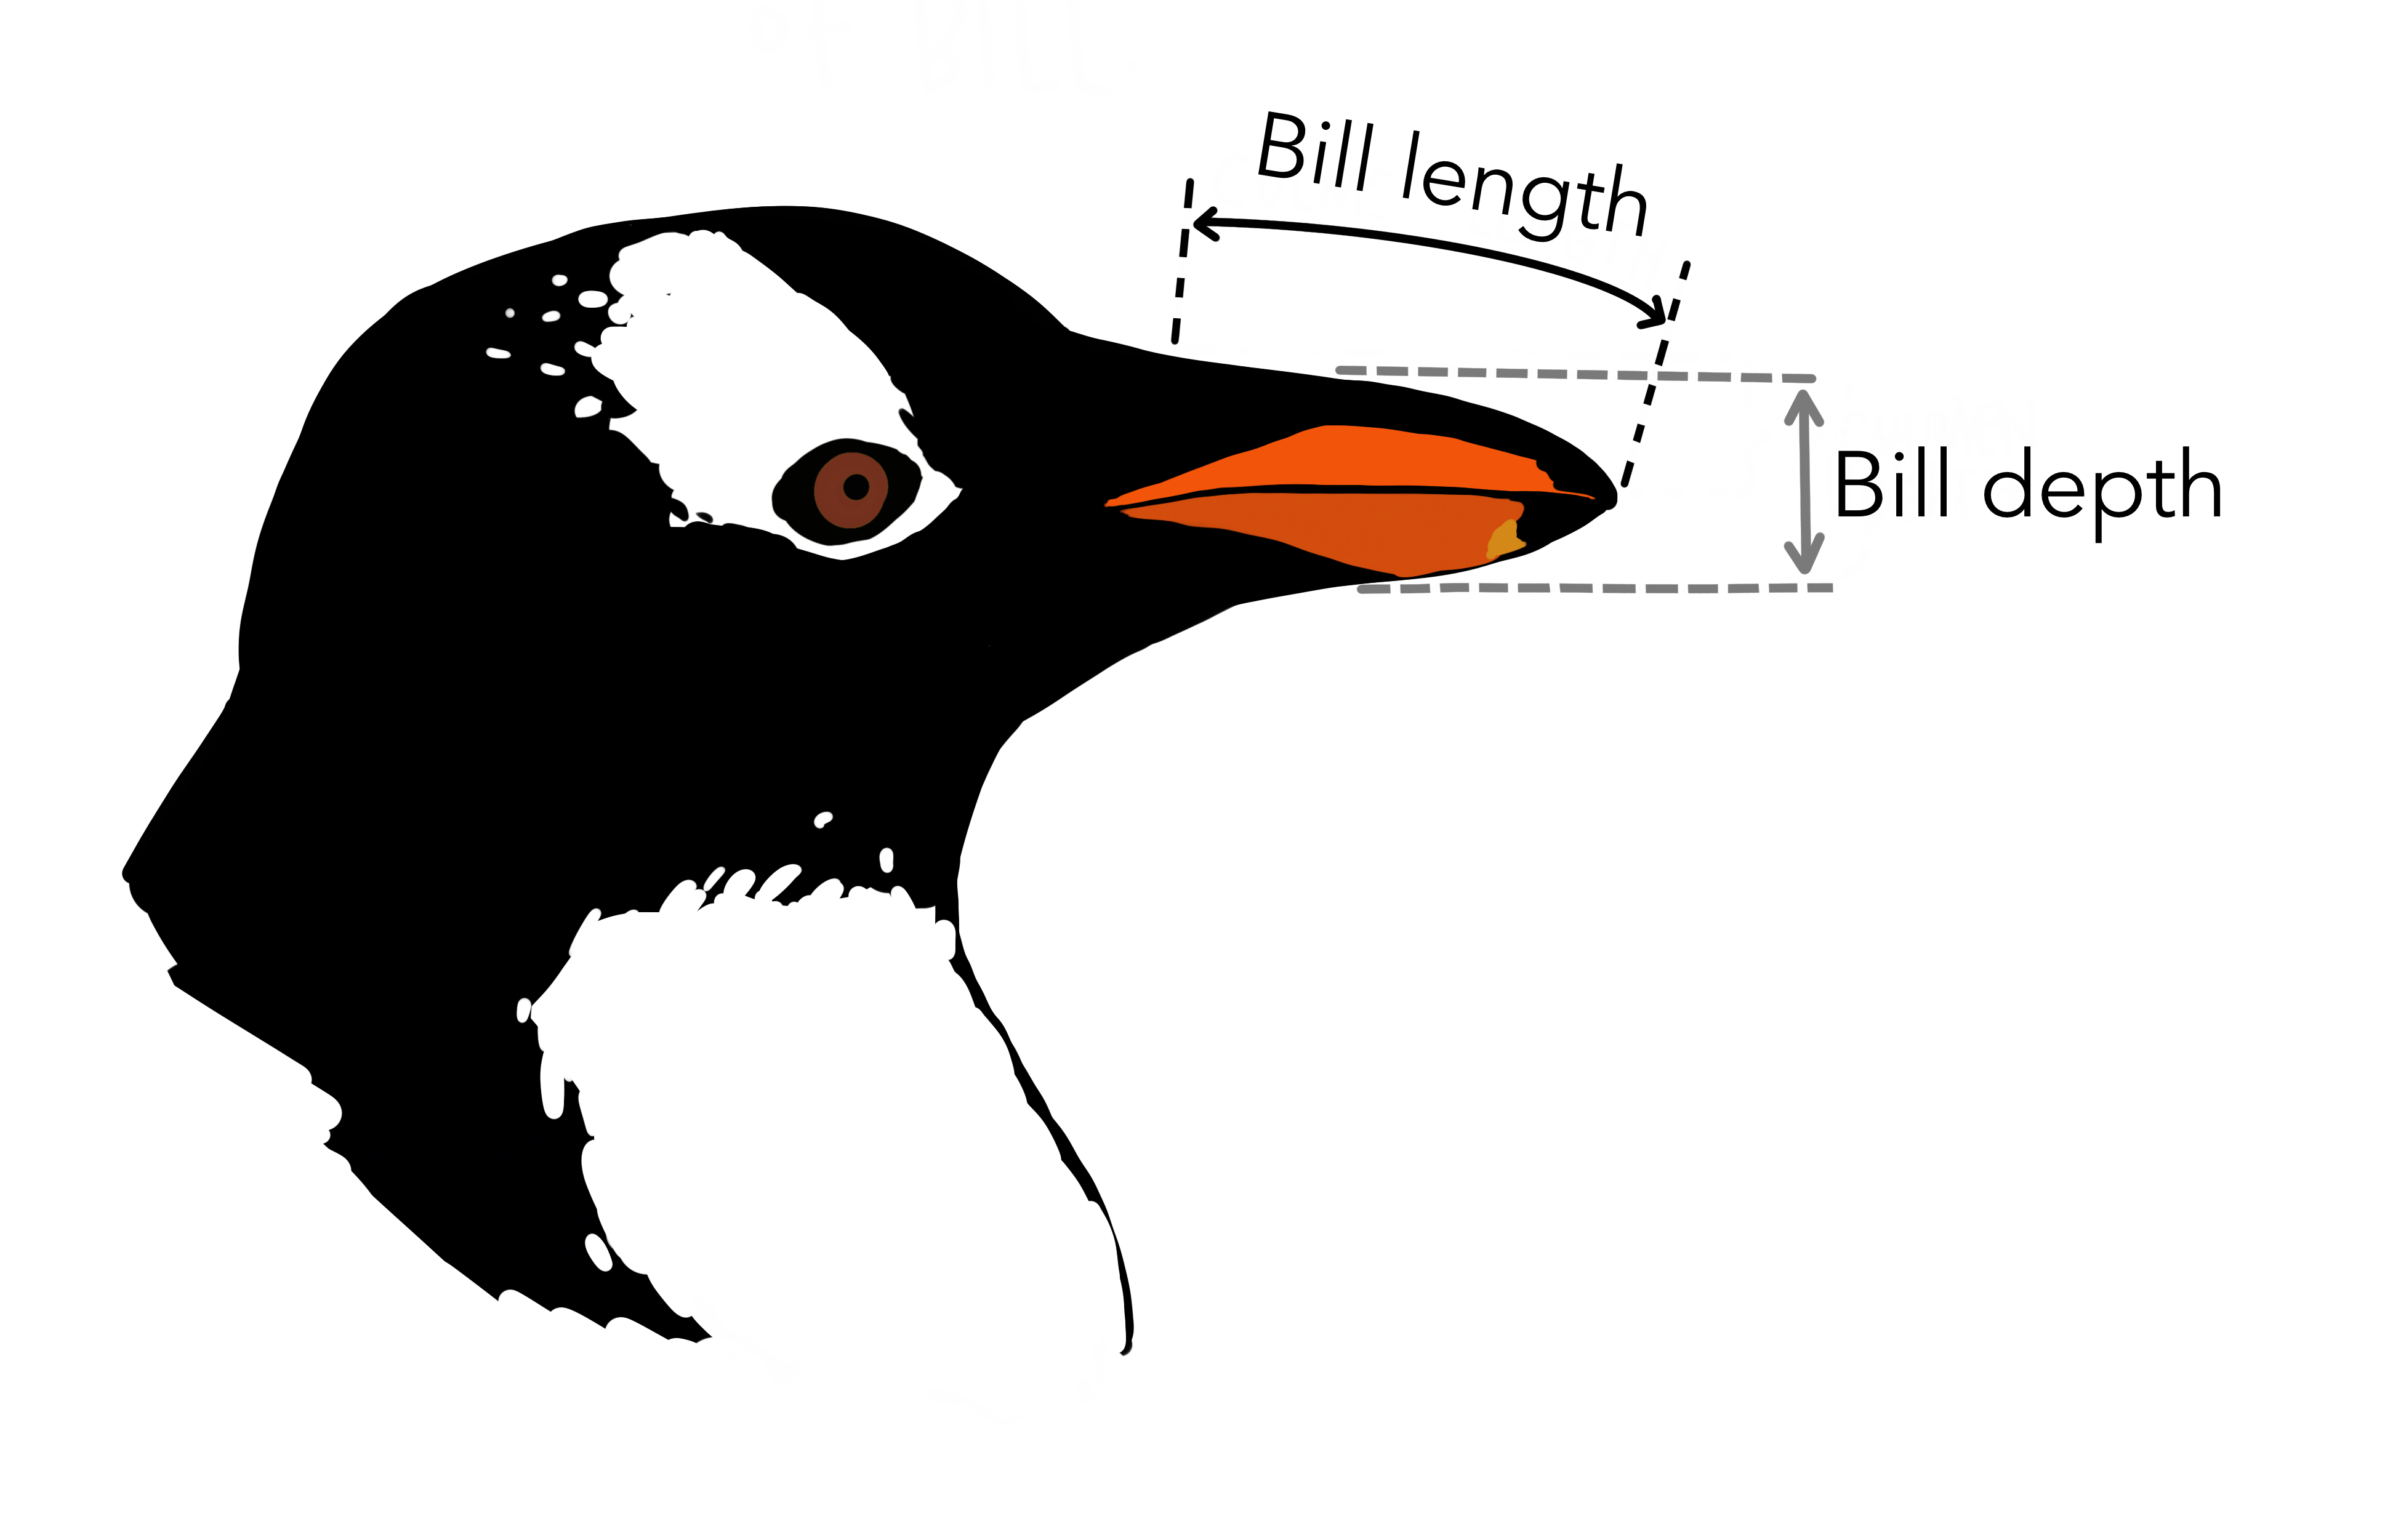
\includegraphics[width=4.16667in,height=\textheight]{chapters/../img/culmen_depth.png}

}

\caption{\label{fig-bill}Ilustración de las variables
\texttt{bill\_length\_mm} y \texttt{bill\_depth\_mm} (Artista
@allison\_horst)}

\end{figure}%

Volviendo a mirar la primera fila de nuestra hoja de datos

\begin{longtable}[]{@{}llllllll@{}}
\toprule\noalign{}
& species & island & bill\_length\_mm & bill\_depth\_mm &
flipper\_length\_mm & body\_mass\_g & sex \\
\midrule\noalign{}
\endhead
\bottomrule\noalign{}
\endlastfoot
0 & Adelie & Torgersen & 39.1 & 18.7 & 181.0 & 3750.0 & MALE \\
\end{longtable}

ahora sabes que el primer pingüino es de la especie Adelie, vive en la
isla Torgensen, las dimensiones de su pico son \(39.1 \times 18.7\)
milímetros, sus alas miden \(181\) milímetros, pesa \(3\) kilos y
\(750\) gramos, y es un macho.

\begin{exercise}[]% 
\protect\hypertarget{exr-data}{}\label{exr-data}%
Describe las características del tercer pingüino del estudio (índice 2).

\end{exercise}

\subsubsection{Valores nulos}\label{valores-nulos}

Fíjate ahora en la columna \texttt{Non-Null\ Count} de la salida del
método \texttt{info()}:

\begin{verbatim}
<class 'pandas.core.frame.DataFrame'>
RangeIndex: 344 entries, 0 to 343
Data columns (total 7 columns):
 #   Column             Non-Null Count  Dtype  
---  ------             --------------  -----  
 0   species            344 non-null    object 
 1   island             344 non-null    object 
 2   bill_length_mm     342 non-null    float64
 3   bill_depth_mm      342 non-null    float64
 4   flipper_length_mm  342 non-null    float64
 5   body_mass_g        342 non-null    float64
 6   sex                333 non-null    object 
dtypes: float64(4), object(3)
memory usage: 18.9+ KB
\end{verbatim}

Los valores nulos o perdidos son valores no disponibles, que no han
podido registrarse, se representan con el símbolo \texttt{NaN}
(iniciales de \emph{Not A Number}).

Si vuelves a mirar las cinco primeras filas de la hoja de datos verás
que para el cuarto pingüino sólo sabemos que es de la especie Adelie y
vive el la isla Torgersen, y se desconocen las otras cinco variables.

\begin{longtable}[]{@{}llllllll@{}}
\toprule\noalign{}
& species & island & bill\_length\_mm & bill\_depth\_mm &
flipper\_length\_mm & body\_mass\_g & sex \\
\midrule\noalign{}
\endhead
\bottomrule\noalign{}
\endlastfoot
3 & Adelie & Torgersen & NaN & NaN & NaN & NaN & NaN \\
\end{longtable}

Los diferentes métodos de la librería \texttt{pandas} contemplan la
posibilidad de que las hojas de datos tengan valores nulos y los tratan
de un forma predeterminada (por ejemplo, la media los ignora por
defecto).

\subsubsection{Tipos de variables}\label{tipos-de-variables}

Las siete variables de nuestra hoja de datos se dividen en dos clases:

\begin{enumerate}
\def\labelenumi{\arabic{enumi}.}
\item
  \texttt{species}, \texttt{island} y \texttt{sex} son \textbf{variables
  categóricas}. Este tipo de variables representan una característica
  cualitativa que puede tomar un número finito y fijo de valores,
  denominados categorías o niveles.
\item
  Las cuatro restantes, \texttt{bill\_length\_mm},
  \texttt{bill\_depth\_mm}, \texttt{flipper\_length\_mm} y
  \texttt{body\_mass\_g} son \textbf{variables numéricas}, que
  representan características cuantitativas que se describen con valores
  numéricos (números enteros o reales).
\end{enumerate}

\texttt{pandas} asigna un tipo a cada variable de una hoja de datos en
función de los valores que presenta, como puede verse en la columna
\texttt{Dtype} de la salida del método \texttt{info()}:

\begin{verbatim}
<class 'pandas.core.frame.DataFrame'>
RangeIndex: 344 entries, 0 to 343
Data columns (total 7 columns):
 #   Column             Non-Null Count  Dtype  
---  ------             --------------  -----  
 0   species            344 non-null    object 
 1   island             344 non-null    object 
 2   bill_length_mm     342 non-null    float64
 3   bill_depth_mm      342 non-null    float64
 4   flipper_length_mm  342 non-null    float64
 5   body_mass_g        342 non-null    float64
 6   sex                333 non-null    object 
dtypes: float64(4), object(3)
memory usage: 18.9+ KB
\end{verbatim}

\subsection{Índice}\label{uxedndice}

Igual que cada columna (variable) en una hoja de datos tiene un nombre,
cada fila (observación) también tiene una etiqueta identificativa. En
nuestra hoja de datos cada uno de los \(344\) pingüinos se identifica
con un número entero de la secuencia 0, 1, \ldots, 333.

\begin{longtable}[]{@{}llllllll@{}}
\toprule\noalign{}
& species & island & bill\_length\_mm & bill\_depth\_mm &
flipper\_length\_mm & body\_mass\_g & sex \\
\midrule\noalign{}
\endhead
\bottomrule\noalign{}
\endlastfoot
0 & Adelie & Torgersen & 39.1 & 18.7 & 181.0 & 3750.0 & MALE \\
1 & Adelie & Torgersen & 39.5 & 17.4 & 186.0 & 3800.0 & FEMALE \\
2 & Adelie & Torgersen & 40.3 & 18.0 & 195.0 & 3250.0 & FEMALE \\
\end{longtable}

\begin{longtable}[]{@{}llllllll@{}}
\toprule\noalign{}
& species & island & bill\_length\_mm & bill\_depth\_mm &
flipper\_length\_mm & body\_mass\_g & sex \\
\midrule\noalign{}
\endhead
\bottomrule\noalign{}
\endlastfoot
341 & Gentoo & Biscoe & 50.4 & 15.7 & 222.0 & 5750.0 & MALE \\
342 & Gentoo & Biscoe & 45.2 & 14.8 & 212.0 & 5200.0 & FEMALE \\
343 & Gentoo & Biscoe & 49.9 & 16.1 & 213.0 & 5400.0 & MALE \\
\end{longtable}

Las etiquetas identificativas de las filas de una hoja de datos forman
su \textbf{índice}. El índice de una hoja de datos de \texttt{pandas} se
registra en su propiedad \texttt{index}.

\begin{Shaded}
\begin{Highlighting}[]
\NormalTok{penguins.index}
\end{Highlighting}
\end{Shaded}

\begin{verbatim}
RangeIndex(start=0, stop=344, step=1)
\end{verbatim}

Si cada pingüino estuviera identificado por un código, podríamos haber
indicado esa variable como índice en el momento de la importación de los
datos. Cuando no se indica el índice de una hoja de datos de forma
explícita, \texttt{pandas} asigna una secuencia de números enteros
comenzando en 0, como ha ocurrido en nuestro caso.

\bookmarksetup{startatroot}

\section{Seleccionar variables}\label{sec-subset-variables}

Al estudiar un conjunto de datos, es frecuente tener que seleccionar los
datos relevantes para responder a las diferentes cuestiones planteadas.

Si por ejemplo queremos saber cuál es el peso máximo de todos los
pingüinos del estudio, seleccionaremos la variable
\texttt{body\_mass\_g} y después calcularemos su máximo.

En esta sección aprenderás los métodos para seleccionar variables de una
hoja de datos.

\subsection{Seleccionar una variable}\label{sec-subset-one-variable}

Utiliza la siguiente instrucción para seleccionar la variable
\texttt{body\_mass\_g}:

\begin{Shaded}
\begin{Highlighting}[]
\NormalTok{mass }\OperatorTok{=}\NormalTok{ penguins[}\StringTok{"body\_mass\_g"}\NormalTok{]}
\end{Highlighting}
\end{Shaded}

\begin{tcolorbox}[enhanced jigsaw, bottomrule=.15mm, colframe=quarto-callout-note-color-frame, toprule=.15mm, leftrule=.75mm, breakable, left=2mm, arc=.35mm, rightrule=.15mm, colback=white, opacityback=0]
\begin{minipage}[t]{5.5mm}
\textcolor{quarto-callout-note-color}{\faInfo}
\end{minipage}%
\begin{minipage}[t]{\textwidth - 5.5mm}

Para seleccionar una sola variable, usa corchetes \texttt{{[}{]}} e
indica el nombre de la columna de interés.

\end{minipage}%
\end{tcolorbox}

Ahora podemos aplicar la función \texttt{max()} para obtener el peso
máximo:

\begin{Shaded}
\begin{Highlighting}[]
\NormalTok{mass.}\BuiltInTok{max}\NormalTok{()}
\end{Highlighting}
\end{Shaded}

\begin{verbatim}
6300.0
\end{verbatim}

Vemos que el pingüino más pesado del estudio pesa \(6\) kilos y \(300\)
gramos.

Podemos realizar las dos operaciones anteriores, seleccionar la variable
\texttt{body\_mass\_g}, y calcular su máximo con una sola instrucción:

\begin{Shaded}
\begin{Highlighting}[]
\NormalTok{penguins[}\StringTok{"body\_mass\_g"}\NormalTok{].}\BuiltInTok{max}\NormalTok{()}
\end{Highlighting}
\end{Shaded}

\begin{verbatim}
6300.0
\end{verbatim}

Obtenemos el mismo resultado de antes.

\begin{exercise}[]% 
\protect\hypertarget{exr-subset-variable-1}{}\label{exr-subset-variable-1}%
Calcula el peso medio de todos los pingüinos (función \texttt{mean()}).

\end{exercise}

\begin{exercise}[]% 
\protect\hypertarget{exr-subset-variable-2}{}\label{exr-subset-variable-2}%
Calcula el valor mínimo para la longitud de las alas de todos los
pingüinos (función \texttt{min()}).

\end{exercise}

\subsection{Seleccionar una lista de
variables}\label{sec-subset-several-variables}

Para seleccionar las dos variables relativas a las dimensiones del pico,
\texttt{bill\_length\_mm} y \texttt{bill\_depth\_mm}, ejecuta la
siguiente instrucción:

\begin{Shaded}
\begin{Highlighting}[]
\NormalTok{bill }\OperatorTok{=}\NormalTok{ penguins[[}\StringTok{"bill\_length\_mm"}\NormalTok{, }\StringTok{"bill\_depth\_mm"}\NormalTok{]]}
\end{Highlighting}
\end{Shaded}

\begin{tcolorbox}[enhanced jigsaw, bottomrule=.15mm, colframe=quarto-callout-note-color-frame, toprule=.15mm, leftrule=.75mm, breakable, left=2mm, arc=.35mm, rightrule=.15mm, colback=white, opacityback=0]
\begin{minipage}[t]{5.5mm}
\textcolor{quarto-callout-note-color}{\faInfo}
\end{minipage}%
\begin{minipage}[t]{\textwidth - 5.5mm}

Para seleccionar una lista de variables, usa corchetes \texttt{{[}{]}}
adicionales para crear la lista con los nombres de las columnas de
interés (los corchetes exteriores indican que se van a seleccionar datos
y los interiores crean la lista).

\end{minipage}%
\end{tcolorbox}

Ahora podemos calcular la media para ambas variables con

\begin{Shaded}
\begin{Highlighting}[]
\NormalTok{bill.mean()}
\end{Highlighting}
\end{Shaded}

\begin{verbatim}
bill_length_mm    43.92193
bill_depth_mm     17.15117
dtype: float64
\end{verbatim}

Vemos que los picos de los pingüinos tienen una longitud media de
\(43.92\) milímetros y una anchura media de \(17.15\) milímetros.

\begin{exercise}[]% 
\protect\hypertarget{exr-subset-variables-3}{}\label{exr-subset-variables-3}%
Calcula el número de observaciones no nulas (función \texttt{count()})
para las variables \texttt{species} y \texttt{body\_mass\_g} con una
sola línea de código.

\end{exercise}

\bookmarksetup{startatroot}

\section{Una variable categórica}\label{una-variable-categuxf3rica}

En este apartado se describen los métodos básicos para explorar y
analizar una variable categórica.

Analizaremos en concreto la variable \texttt{species} de nuestra hoja de
datos, para conocer la distribución de los pingüinos por especies.

Comenzamos seleccionando la variable de interés en nuestra hoja de
datos. Almacenamos el resultado en un nuevo objeto de nombre
\texttt{species}.

\begin{Shaded}
\begin{Highlighting}[]
\NormalTok{species }\OperatorTok{=}\NormalTok{ penguins[}\StringTok{"species"}\NormalTok{]}
\end{Highlighting}
\end{Shaded}

\subsection{\texorpdfstring{El método
\texttt{describe()}}{El método describe()}}\label{sec-1categorical-describe}

Para obtener la información más relevante sobre la distribución de las
especies de pingüinos aplicamos a \texttt{species} el método
\texttt{describe()}:

\begin{Shaded}
\begin{Highlighting}[]
\NormalTok{species.describe()}
\end{Highlighting}
\end{Shaded}

\begin{verbatim}
count        344
unique         3
top       Adelie
freq         152
Name: species, dtype: object
\end{verbatim}

De la salida anterior obtenemos la siguiente información sobre la
variable \texttt{species}:

\begin{longtable}[]{@{}
  >{\raggedright\arraybackslash}p{(\columnwidth - 2\tabcolsep) * \real{0.4167}}
  >{\raggedright\arraybackslash}p{(\columnwidth - 2\tabcolsep) * \real{0.5833}}@{}}
\toprule\noalign{}
\begin{minipage}[b]{\linewidth}\raggedright
Fragmento de la salida
\end{minipage} & \begin{minipage}[b]{\linewidth}\raggedright
Significado
\end{minipage} \\
\midrule\noalign{}
\endhead
\bottomrule\noalign{}
\endlastfoot
\texttt{count\ \ \ 344} & Hay \(344\) valores no nulos, así que se
conoce la especie de todos los pingüinos del estudio. \\
\texttt{unique\ \ \ \ 3} & La variable toma tres valores diferentes, es
decir, hay tres categorías (las tres especies Adelie, Chinstrap y
Gentooo). \\
\texttt{top\ \ Adelie} & La categoría \texttt{top} o más frecuente, es
decir, la especie más numerosa es la especie Adelie. \\
\texttt{freq\ \ \ \ 152} & El número de pingüinos de la especie Adelie
(la categoría \texttt{top}) es \(152\). \\
\end{longtable}

\begin{exercise}[]% 
\protect\hypertarget{exr-1categorical-describe}{}\label{exr-1categorical-describe}%
Utiliza el método \texttt{describe()} para obtener información sobre la
distribución de los pingüinos por islas.

\end{exercise}

\subsection{Tabla de recuentos}\label{sec-value-counts}

Ya sabemos que la especie más numerosa es Adelie, con \(152\) pingüinos,
pero aún no sabemos cuántos pingüinos hay de las otras dos especies,
Chinstrap y Gentoo. Para obtener una tabla con el número de pingüinos de
cada especie usamos la función \texttt{value\_counts()}:

\begin{Shaded}
\begin{Highlighting}[]
\NormalTok{species.value\_counts()}
\end{Highlighting}
\end{Shaded}

\begin{verbatim}
species
Adelie       152
Gentoo       124
Chinstrap     68
Name: count, dtype: int64
\end{verbatim}

Ahora sabemos que la segunda especie más numerosa es Gentoo, con 124
ejemplares, y que solo hay 68 pingüinos de la especie Chinstrap.

\begin{exercise}[]% 
\protect\hypertarget{exr-1categorial-sex-counts}{}\label{exr-1categorial-sex-counts}%
Determina el número total de hembras y de machos.

\end{exercise}

\subsection{Diagrama de recuentos}\label{diagrama-de-recuentos}

Un \textbf{diagrama de recuentos} asocia a cada categoría una barra de
longitud igual al número de observaciones en esa categoría.

Para realizar un diagrama del recuento de pingüinos por especie usamos
la función \texttt{countplot()} del paquete \texttt{seaborn}

\begin{Shaded}
\begin{Highlighting}[]
\NormalTok{sns.countplot(data}\OperatorTok{=}\NormalTok{penguins, x}\OperatorTok{=}\StringTok{"species"}\NormalTok{)}\OperatorTok{;}
\end{Highlighting}
\end{Shaded}

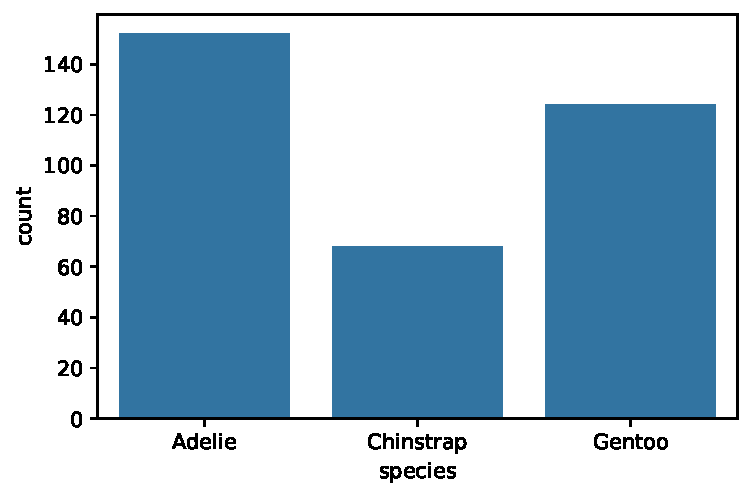
\includegraphics{chapters/1categorical_files/figure-pdf/cell-6-output-1.pdf}

\begin{tcolorbox}[enhanced jigsaw, bottomrule=.15mm, colframe=quarto-callout-note-color-frame, toprule=.15mm, leftrule=.75mm, breakable, left=2mm, arc=.35mm, rightrule=.15mm, colback=white, opacityback=0]
\begin{minipage}[t]{5.5mm}
\textcolor{quarto-callout-note-color}{\faInfo}
\end{minipage}%
\begin{minipage}[t]{\textwidth - 5.5mm}

Si quitas el punto y coma \texttt{;} al final de la instrucción anterior
aparecerá el mensaje

\texttt{\textless{}AxesSubplot:xlabel=\textquotesingle{}count\textquotesingle{},\ ylabel=\textquotesingle{}species\textquotesingle{}\textgreater{}}

en la salida antes del gráfico.

Al terminar una instrucción con punto y coma \texttt{;} se inhibe la
impresión de la salida.

\end{minipage}%
\end{tcolorbox}

Nota que las alturas de las barras en el gráfico anterior coindicen con
los recuentos que hemos calculado en el apartado anterior con
\texttt{value\_counts()}.

A veces es preferible usar barras horizontales, porque se tiene más
espacio para las etiquetas de las categorías.

\begin{Shaded}
\begin{Highlighting}[]
\NormalTok{sns.countplot(data}\OperatorTok{=}\NormalTok{penguins, y}\OperatorTok{=}\StringTok{"species"}\NormalTok{)}\OperatorTok{;}
\end{Highlighting}
\end{Shaded}

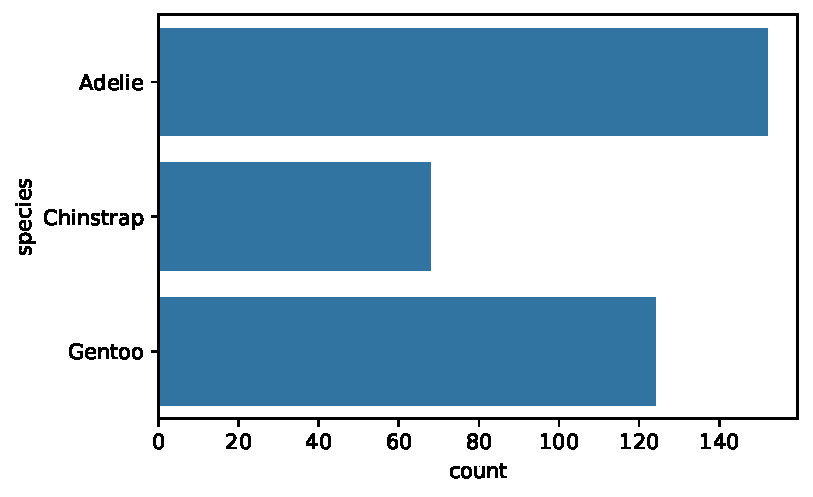
\includegraphics{chapters/1categorical_files/figure-pdf/cell-7-output-1.pdf}

\begin{tcolorbox}[enhanced jigsaw, bottomrule=.15mm, colframe=quarto-callout-note-color-frame, toprule=.15mm, leftrule=.75mm, breakable, left=2mm, arc=.35mm, rightrule=.15mm, colback=white, opacityback=0]
\begin{minipage}[t]{5.5mm}
\textcolor{quarto-callout-note-color}{\faInfo}
\end{minipage}%
\begin{minipage}[t]{\textwidth - 5.5mm}

Para realizar un diagrama de recuentos de las categorías de una variable
categórica, usa la función \texttt{countplot()} de\texttt{seaborn}. E
indica:

\begin{itemize}
\tightlist
\item
  El nombre de la hoja de datos como valor del argumento \texttt{data}.
\item
  El nombre de la variable categórica como valor del argumento
  \texttt{x} si quieres barras verticales, o como valor del argumento
  \texttt{y} si quieres barras horizontales.
\end{itemize}

\end{minipage}%
\end{tcolorbox}

\begin{exercise}[]% 
\protect\hypertarget{exr-1categorial-countplot-vertical}{}\label{exr-1categorial-countplot-vertical}%
Crea un diagrama de recuentos para el número de hembras y machos, con
barras verticales.

\end{exercise}

\begin{exercise}[]% 
\protect\hypertarget{exr-1categorial-sns-countplot}{}\label{exr-1categorial-sns-countplot}%
Crea un diagrama de recuentos para el número de pingüinos en cada isla,
con barras horizontales.

\end{exercise}

\subsection{Personalización de los gráficos
(opcional)}\label{personalizaciuxf3n-de-los-gruxe1ficos-opcional}

Los gráficos de la librería \texttt{seaborn} admiten muchas opciones
para personalizar su aspecto cambiando por ejemplo los colores, los
rótulos de los ejes, etc.

La personalización de los gráficos no carece de importancia, siendo
especialmente relevante dar títulos descriptivos a los ejes. Pero en
esta práctica nos centraremos en los procedimientos para realizar los
gráficos y en la mayoría de ocasiones omitiremos los detalles de
personalización de los mismos, que pueden consultarse en la
documentación de \texttt{seaborn}.

En este apartado se da una muestra de las opciones para personalizar los
diagramas de recuentos que se han presentado en el apartado anterior. Se
trata de un apartado opcional y puedes por ahora omitir su lectura y
volver a él al final de la práctica.

\subsubsection{Colores}\label{colores}

Si quieres cambiar el color de las barras usa el argumento
\texttt{color}:

\begin{Shaded}
\begin{Highlighting}[]
\NormalTok{sns.countplot(data}\OperatorTok{=}\NormalTok{penguins, x}\OperatorTok{=}\StringTok{"species"}\NormalTok{, color}\OperatorTok{=}\StringTok{"coral"}\NormalTok{)}\OperatorTok{;}
\end{Highlighting}
\end{Shaded}

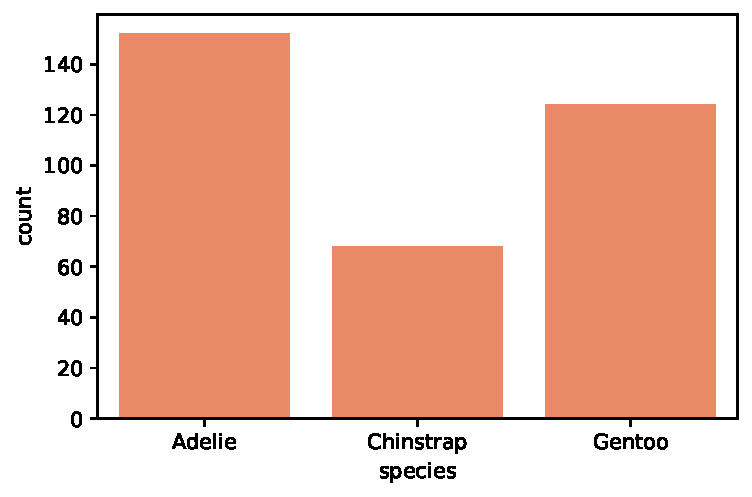
\includegraphics{chapters/1categorical_files/figure-pdf/cell-8-output-1.pdf}

Puedes ver los colores disponibles
\href{https://matplotlib.org/stable/tutorials/colors/colors.html}{aquí}.

Para utilizar un color diferente para la barra de cada categoría usa el
argumento \texttt{hue}:

\begin{Shaded}
\begin{Highlighting}[]
\NormalTok{sns.countplot(data}\OperatorTok{=}\NormalTok{penguins, x}\OperatorTok{=}\StringTok{"species"}\NormalTok{, hue}\OperatorTok{=}\StringTok{"species"}\NormalTok{)}\OperatorTok{;}
\end{Highlighting}
\end{Shaded}

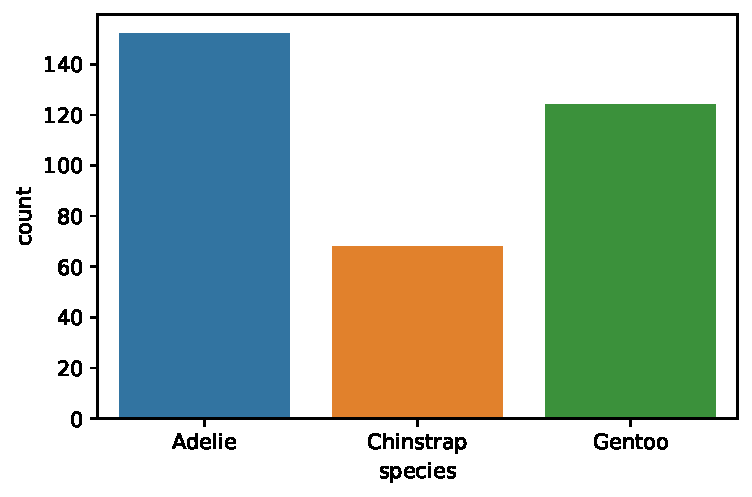
\includegraphics{chapters/1categorical_files/figure-pdf/cell-9-output-1.pdf}

También se puede indicar una secuencia de colores personalizada usando
el argumento \texttt{palette}:

\begin{Shaded}
\begin{Highlighting}[]
\NormalTok{sns.countplot(data}\OperatorTok{=}\NormalTok{penguins, x}\OperatorTok{=}\StringTok{"species"}\NormalTok{, hue}\OperatorTok{=}\StringTok{"species"}\NormalTok{, palette}\OperatorTok{=}\NormalTok{[}\StringTok{"steelblue"}\NormalTok{, }\StringTok{"coral"}\NormalTok{, }\StringTok{"gold"}\NormalTok{])}\OperatorTok{;}
\end{Highlighting}
\end{Shaded}

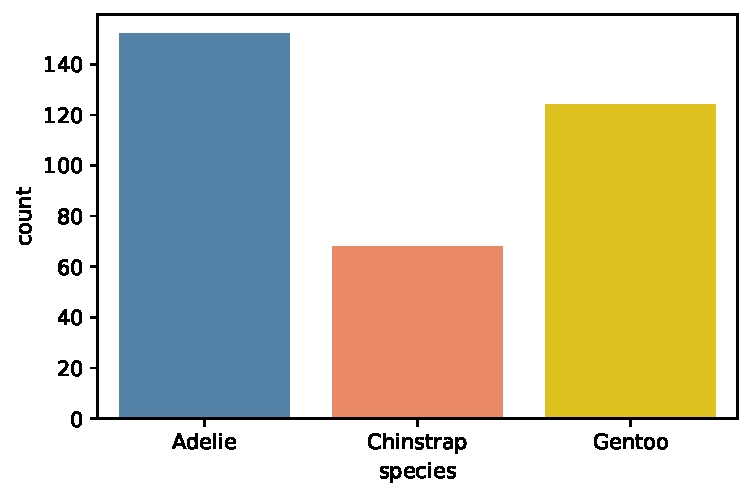
\includegraphics{chapters/1categorical_files/figure-pdf/cell-10-output-1.pdf}

Como valor para \texttt{palette} se puede indicar una lista de colores,
como en el ejemplo anterior, o el nombre de una de las paletes
predefinidas (\texttt{deep}, \texttt{muted}, \texttt{pastel},
\texttt{bright}, \texttt{dark} y \texttt{colorblind}), como en el
siguiente ejemplo:

\begin{Shaded}
\begin{Highlighting}[]
\NormalTok{sns.countplot(data}\OperatorTok{=}\NormalTok{penguins, x}\OperatorTok{=}\StringTok{"species"}\NormalTok{, hue}\OperatorTok{=}\StringTok{"species"}\NormalTok{, palette}\OperatorTok{=}\StringTok{"colorblind"}\NormalTok{)}\OperatorTok{;}
\end{Highlighting}
\end{Shaded}

\subsubsection{Rótulos}\label{ruxf3tulos}

Con el siguiente código personalizamos los títulos de los ejes y damos
un título global al gráfico

\begin{Shaded}
\begin{Highlighting}[]
\NormalTok{ax }\OperatorTok{=}\NormalTok{ sns.countplot(data}\OperatorTok{=}\NormalTok{penguins, x}\OperatorTok{=}\StringTok{"species"}\NormalTok{)}
\NormalTok{ax.}\BuiltInTok{set}\NormalTok{(}
\NormalTok{    title}\OperatorTok{=}\StringTok{"Número de pingüinos de cada especie"}\NormalTok{,}
\NormalTok{    xlabel}\OperatorTok{=}\StringTok{"Especie"}\NormalTok{, }
\NormalTok{    ylabel}\OperatorTok{=}\StringTok{"Número de pingüinos"}
\NormalTok{)}\OperatorTok{;}
\end{Highlighting}
\end{Shaded}

\begin{center}
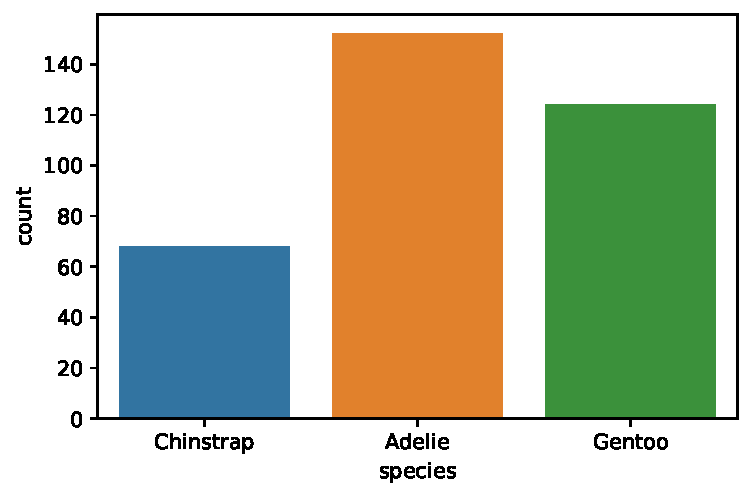
\includegraphics{chapters/1categorical_files/figure-pdf/cell-12-output-1.pdf}
\end{center}

\subsubsection{Orden de los niveles}\label{orden-de-los-niveles}

Si te fijas en los gráficos que has hecho hasta ahora, apreciarás que
las categorías aparecen en los gráficos en el mismo orden en el que
aparecen en las filas de la hoja de datos.

Si quieres un orden personalizado para las categorías puedes usar el
argumento \texttt{order}, como en el siguiente ejemplo:

\begin{Shaded}
\begin{Highlighting}[]
\NormalTok{sns.countplot(data}\OperatorTok{=}\NormalTok{penguins, x}\OperatorTok{=}\StringTok{"species"}\NormalTok{, order }\OperatorTok{=}\NormalTok{ [}\StringTok{\textquotesingle{}Chinstrap\textquotesingle{}}\NormalTok{, }\StringTok{\textquotesingle{}Adelie\textquotesingle{}}\NormalTok{, }\StringTok{\textquotesingle{}Gentoo\textquotesingle{}}\NormalTok{])}\OperatorTok{;}
\end{Highlighting}
\end{Shaded}

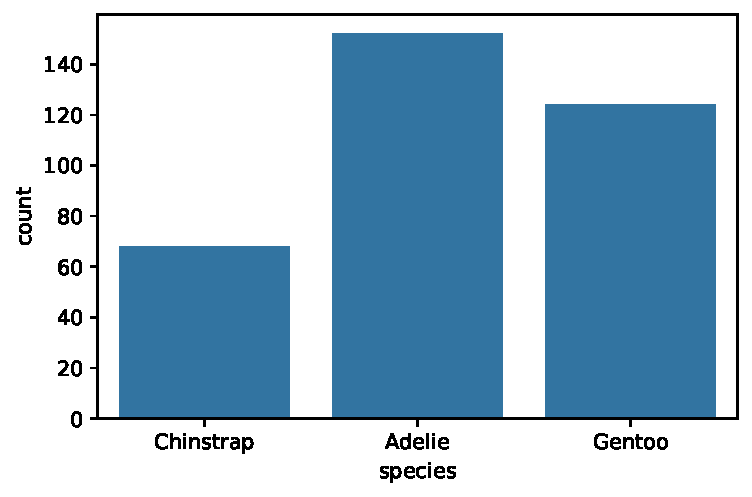
\includegraphics{chapters/1categorical_files/figure-pdf/cell-13-output-1.pdf}

Con el siguiente código ordenamos las categorías de mayor a menor
frecuencia.

\begin{Shaded}
\begin{Highlighting}[]
\NormalTok{sns.countplot(data}\OperatorTok{=}\NormalTok{penguins, x}\OperatorTok{=}\StringTok{"species"}\NormalTok{, order }\OperatorTok{=}\NormalTok{ species.value\_counts().index)}\OperatorTok{;}
\end{Highlighting}
\end{Shaded}

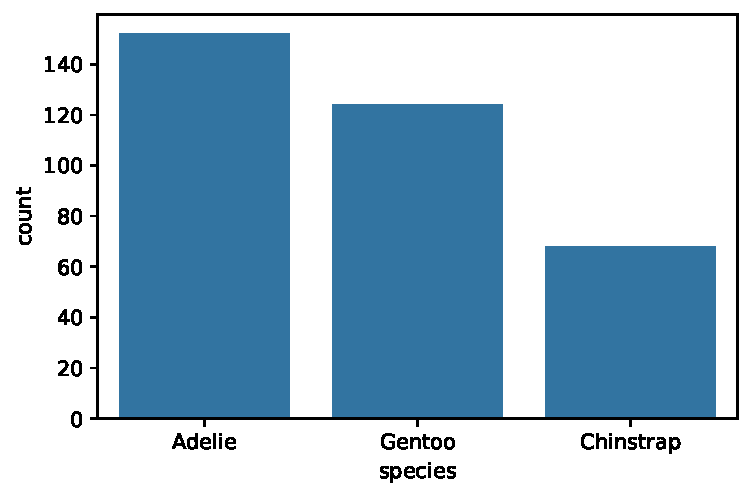
\includegraphics{chapters/1categorical_files/figure-pdf/cell-14-output-1.pdf}

\bookmarksetup{startatroot}

\section{Una variable numérica}\label{sec-1numerical}

Igual que en el apartado anterior estudiamos una variable categórica, en
este apartado se describen los métodos básicos para explorar y analizar
una variable numérica.

Analizaremos en concreto la variable \texttt{body\_mass\_g} de nuestra
hoja de datos, para conocer la distribución de los pesos de los
pingüinos.

Empezamos seleccionando la variable de interés y almacenando el
resultado en un nuevo objeto de nombre \texttt{mass}.

\begin{Shaded}
\begin{Highlighting}[]
\NormalTok{mass }\OperatorTok{=}\NormalTok{ penguins[}\StringTok{"body\_mass\_g"}\NormalTok{]}
\end{Highlighting}
\end{Shaded}

\subsection{\texorpdfstring{El método
\texttt{describe()}}{El método describe()}}\label{sec-1numerical-describe}

El método \texttt{describe()} que usamos en la sección anterior para una
variable categórica, también puede aplicarse a variables numéricas.

Si lo aplicamos a \texttt{mass} obtenemos el siguiente resultado:

\begin{Shaded}
\begin{Highlighting}[]
\NormalTok{mass.describe()}
\end{Highlighting}
\end{Shaded}

\begin{verbatim}
count     342.000000
mean     4201.754386
std       801.954536
min      2700.000000
25%      3550.000000
50%      4050.000000
75%      4750.000000
max      6300.000000
Name: body_mass_g, dtype: float64
\end{verbatim}

La información que obtenemos de la salida anterior sobre la distribución
del peso de los pingüinos es la siguiente:

\begin{longtable}[]{@{}
  >{\raggedright\arraybackslash}p{(\columnwidth - 2\tabcolsep) * \real{0.4545}}
  >{\raggedright\arraybackslash}p{(\columnwidth - 2\tabcolsep) * \real{0.5455}}@{}}
\toprule\noalign{}
\begin{minipage}[b]{\linewidth}\raggedright
Fragmento de la salida
\end{minipage} & \begin{minipage}[b]{\linewidth}\raggedright
Significado
\end{minipage} \\
\midrule\noalign{}
\endhead
\bottomrule\noalign{}
\endlastfoot
\texttt{count\ \ \ \ \ 342.000000} & Hay 342 valores no nulos, así que
no se conoce el peso de dos pingüinos. \\
\texttt{mean\ \ \ \ \ 4201.754386} & El peso medio de los pingüinos es
\(4\) kilogramos y \(201\) gramos. \\
\texttt{std\ \ \ \ \ \ \ 801.954536} & La desviación estandar del peso
de los pinguinos es \(801\) gramos. \\
\texttt{min\ \ \ \ \ \ 2700.000000} & El pingüino que menos pesa, pesa
\(2\) kilos y \(700\) gramos. \\
\texttt{25\%\ \ \ \ \ \ 3550.000000} & El \(25\%\) de los pingüinos pesa
menos de \(3\) kilos y \(550\) gramos (y el \(75\%\) restante más). Este
valor se conoce como \textbf{cuantil 0.25} o \textbf{primer cuartil}. \\
\texttt{50\%\ \ \ \ \ \ 4050.000000} & El \(50\%\) de los pingüinos pesa
menos de \(4\) kilos y \(50\) gramos (y el \(50\%\) restante más). Este
valor se llama \textbf{cuantil 0.5}, \textbf{segundo cuartil} o
\textbf{mediana}. \\
\texttt{75\%\ \ \ \ \ \ 4750.000000} & El \(75\%\) de los pingüinos pesa
menos de \(4\) kilos y \(750\) gramos (y el \(25\%\) restante más). Este
valor se llama \textbf{cuantil 0.75} o \textbf{tercer cuartil}. \\
\texttt{max\ \ \ \ \ \ 6300.000000} & El pingüino que más pesa, pesa
\(6\) kilos y \(300\) gramos. \\
\end{longtable}

\begin{exercise}[]% 
\protect\hypertarget{exr-1numerical-describe}{}\label{exr-1numerical-describe}%
Utiliza el método \texttt{describe()} para obtener información sobre la
distribución de la longitud de las alas de los pingüinos.

\end{exercise}

\subsection{Histograma}\label{sec-1numerical-histogram}

Los \textbf{histogramas} son uno de los gráficos más comunes e
informativos para describir la distribución de una variable continua.
Para crear un histograma se representa en el eje x el rango de valores
de la variable, se divide ese rango en intervalos de la misma longitud,
y se dibuja para cada intervalo una barra de altura igual al número de
valores que caen en ese intervalo.

El siguiente código crea un histograma para el peso de los pingüinos:

\begin{Shaded}
\begin{Highlighting}[]
\NormalTok{sns.histplot(data}\OperatorTok{=}\NormalTok{penguins, x}\OperatorTok{=}\StringTok{"body\_mass\_g"}\NormalTok{)}\OperatorTok{;}
\end{Highlighting}
\end{Shaded}

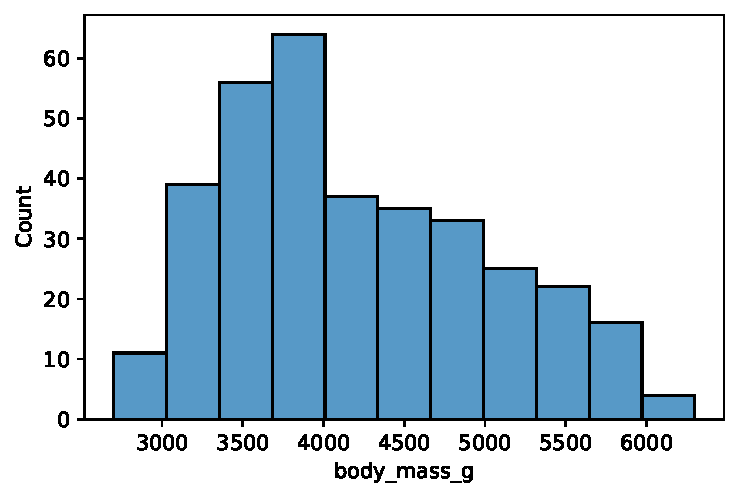
\includegraphics{chapters/1numerical_files/figure-pdf/cell-5-output-1.pdf}

\begin{tcolorbox}[enhanced jigsaw, bottomrule=.15mm, colframe=quarto-callout-note-color-frame, toprule=.15mm, leftrule=.75mm, breakable, left=2mm, arc=.35mm, rightrule=.15mm, colback=white, opacityback=0]
\begin{minipage}[t]{5.5mm}
\textcolor{quarto-callout-note-color}{\faInfo}
\end{minipage}%
\begin{minipage}[t]{\textwidth - 5.5mm}

Para realizar un histograma usa la función \texttt{histplot()} del
paquete \texttt{seaborn}, e indica:

\begin{itemize}
\tightlist
\item
  El nombre de la hoja de datos como valor del argumento \texttt{data}.
\item
  El nombre de la variable como valor del argumento \texttt{x}.
\end{itemize}

\end{minipage}%
\end{tcolorbox}

\begin{exercise}[]% 
\protect\hypertarget{exr-1numerical-histplot}{}\label{exr-1numerical-histplot}%
Realiza un histograma para la longitud de las alas de los pingüinos.

\end{exercise}

\subsection{Diagrama de caja y bigotes}\label{sec-1numerical-boxplot}

Otro tipo de gráficos para variables numéricas son los llamados
\textbf{diagramas de caja} o \textbf{de caja y bigotes}.

Ejecuta el siguiente código para crear un diagrama de caja y bigotes
para el peso de los pingüinos.

\begin{Shaded}
\begin{Highlighting}[]
\NormalTok{sns.boxplot(data}\OperatorTok{=}\NormalTok{penguins, y}\OperatorTok{=}\StringTok{"body\_mass\_g"}\NormalTok{)}\OperatorTok{;}
\end{Highlighting}
\end{Shaded}

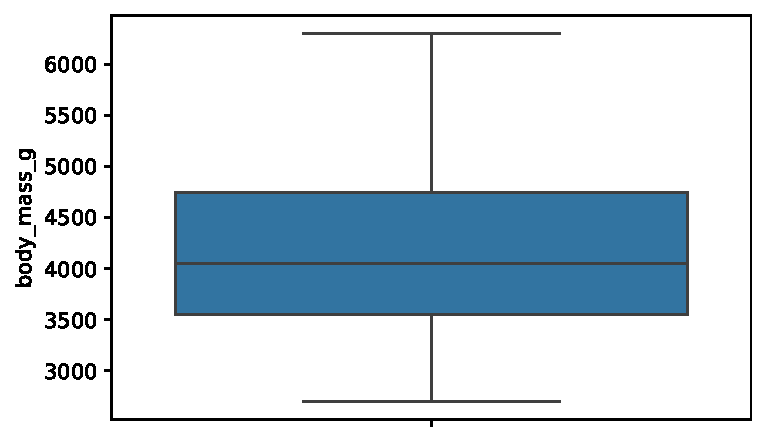
\includegraphics{chapters/1numerical_files/figure-pdf/cell-6-output-1.pdf}

La caja se construye usando los cuartiles de la variable.

Y los bigotes se extienden desde los extremos de la caja hasta los
valores mínimo y máximo, exceptuando los valores que se clasifican como
\textbf{outliers}.

\begin{tcolorbox}[enhanced jigsaw, bottomrule=.15mm, colframe=quarto-callout-note-color-frame, toprule=.15mm, leftrule=.75mm, breakable, left=2mm, arc=.35mm, rightrule=.15mm, colback=white, opacityback=0]
\begin{minipage}[t]{5.5mm}
\textcolor{quarto-callout-note-color}{\faInfo}
\end{minipage}%
\begin{minipage}[t]{\textwidth - 5.5mm}

Para realizar un diagrama de caja y bigotes usa la función
\texttt{boxplot()} del paquete \texttt{seaborn} e indica:

\begin{itemize}
\tightlist
\item
  El nombre de la hoja de datos como valor del argumento \texttt{data}.
\item
  El nombre de la variable como valor del argumento \texttt{y}.
\end{itemize}

\end{minipage}%
\end{tcolorbox}

\begin{exercise}[]% 
\protect\hypertarget{exr-1numerical-boxplot}{}\label{exr-1numerical-boxplot}%
Realiza un diagrama de caja y bigotes para la longitud de las alas de
los pingüinos.

\end{exercise}

\bookmarksetup{startatroot}

\section{Agrupar por categorías}\label{sec-groupby}

En la Sección~\ref{sec-head-tail} visualizamos los datos de los cinco
primeros pingüinos con la instrucción

\begin{Shaded}
\begin{Highlighting}[]
\NormalTok{penguins.head(}\DecValTok{5}\NormalTok{)}
\end{Highlighting}
\end{Shaded}

Y en la Sección~\ref{sec-subset-one-variable} calculamos el peso máximo
de todos los pingüinos con la orden

\begin{Shaded}
\begin{Highlighting}[]
\NormalTok{penguins[}\StringTok{"body\_mass\_g"}\NormalTok{].}\BuiltInTok{max}\NormalTok{()}
\end{Highlighting}
\end{Shaded}

Ahora nos planteamos realizar las operaciones anteriores, pero para cada
especie de pingüinos (Adelie, Chinstrap y Gentoo), es decir, queremos:

\begin{itemize}
\tightlist
\item
  Ver los datos de los primeros pingüinos de cada una de las tres
  especies.
\item
  Calcular el peso máximo en cada una de las tres especies de pingüinos.
\end{itemize}

\texttt{pandas} proporciona el método \texttt{groupby()} para resolver
este tipo de problemas.

El método \texttt{groupby()} divide una hoja de datos en los grupos o
categorías definidos por una variable categórica (en nuestro caso las
tres especies dadas por la variable \texttt{species}), de forma que al
realizar una operación (como \texttt{head()} o \texttt{máx()}) en la
hoja de datos por grupos, obtendremos el resultado de la operación en
cada uno de los grupos (en nuestro caso en cada especie).

\begin{figure}[tbph]

{\centering 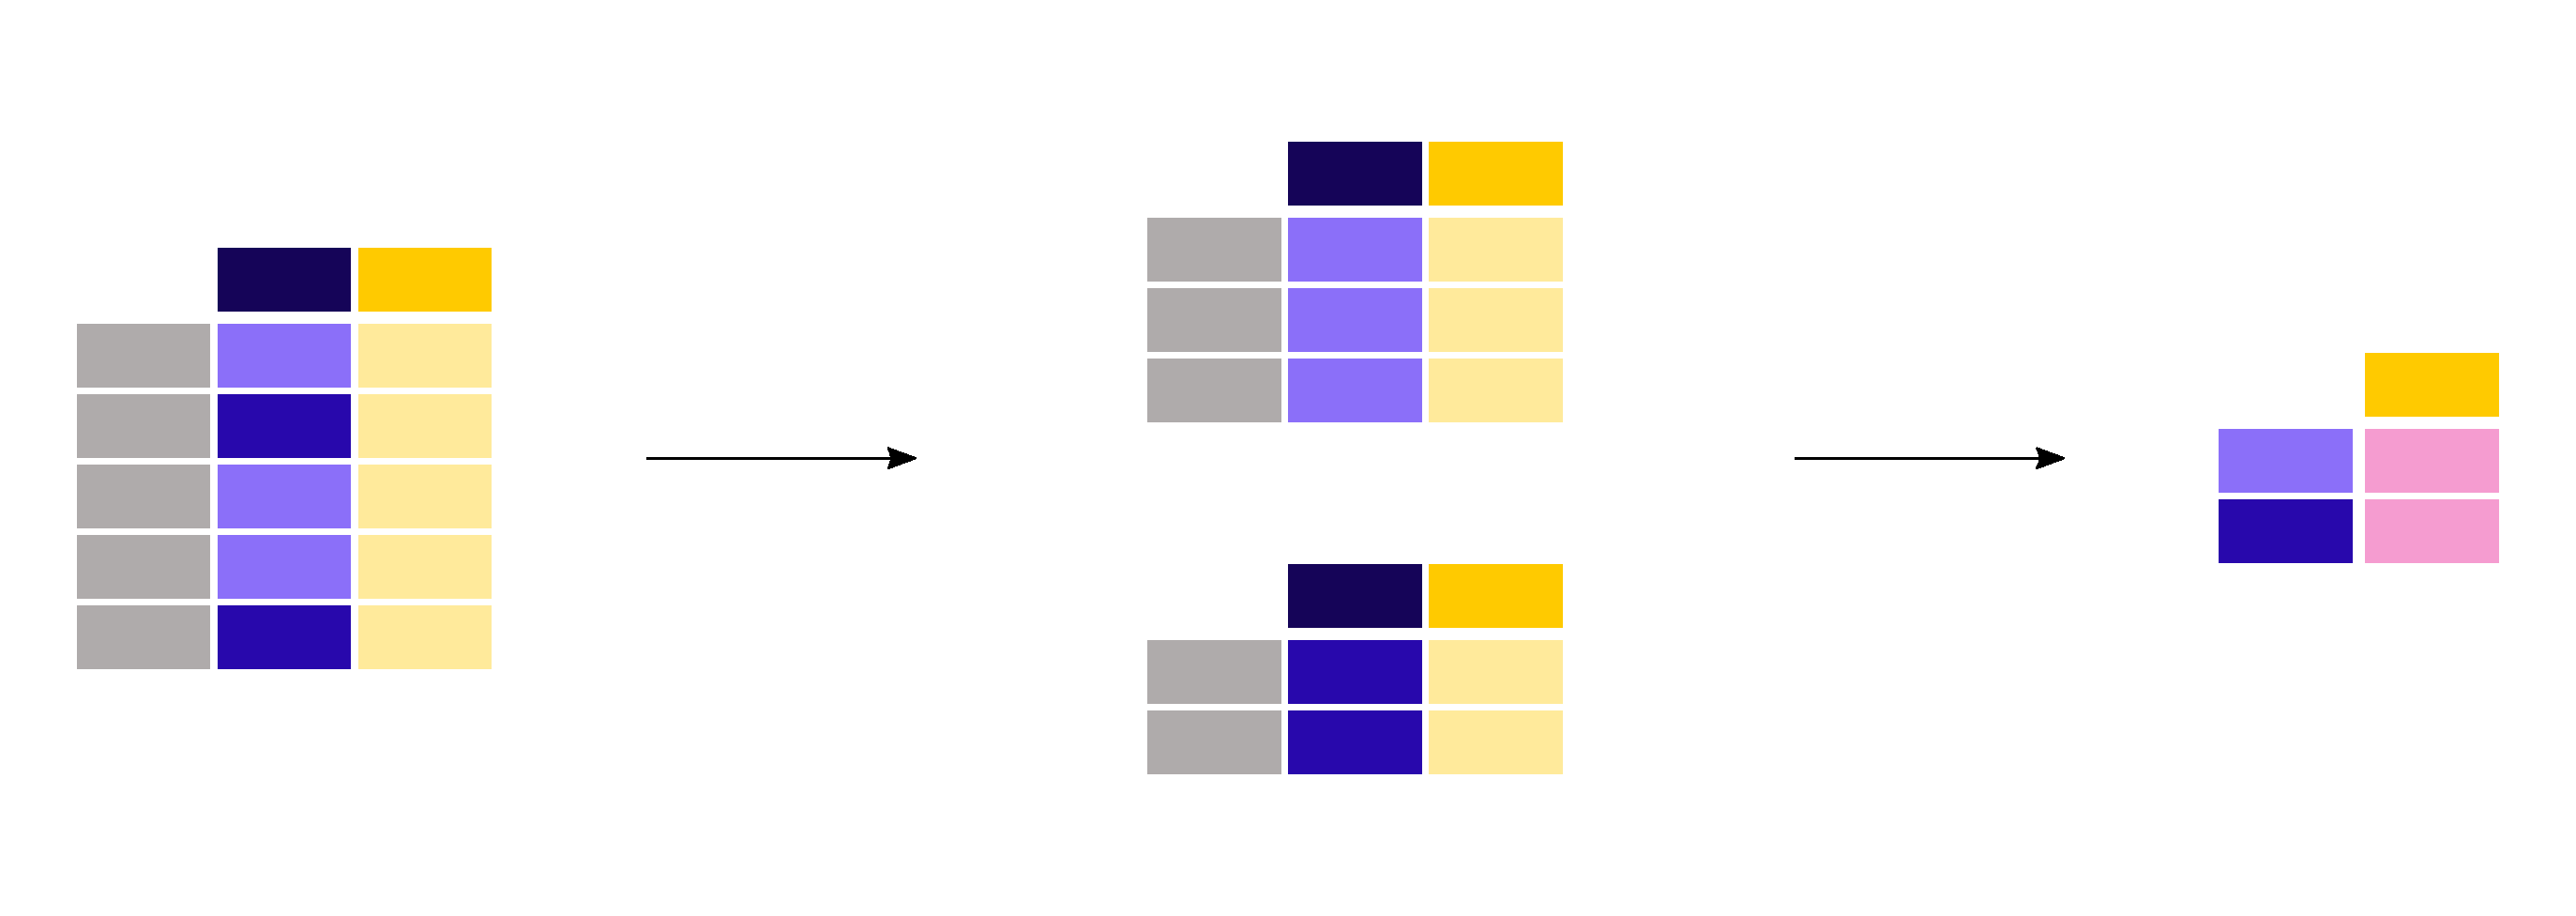
\includegraphics{index_files/mediabag/chapters/../img/06_groupby.pdf}

}

\caption{Ilustración del método \texttt{groupby()} en el manual de
\texttt{pandas}}

\end{figure}%

\subsection*{Ejemplo 1: Primeras filas de cada
especie}\label{ejemplo-1-primeras-filas-de-cada-especie}
\addcontentsline{toc}{subsection}{Ejemplo 1: Primeras filas de cada
especie}


Para ver los datos de los tres primeros pingüinos de cada especie,
ejecuta la instrucción siguiente:

\begin{Shaded}
\begin{Highlighting}[]
\NormalTok{penguins.groupby(}\StringTok{"species"}\NormalTok{).head(}\DecValTok{3}\NormalTok{)}
\end{Highlighting}
\end{Shaded}

\begin{longtable}[]{@{}llllllll@{}}
\toprule\noalign{}
& species & island & bill\_length\_mm & bill\_depth\_mm &
flipper\_length\_mm & body\_mass\_g & sex \\
\midrule\noalign{}
\endhead
\bottomrule\noalign{}
\endlastfoot
0 & Adelie & Torgersen & 39.1 & 18.7 & 181.0 & 3750.0 & MALE \\
1 & Adelie & Torgersen & 39.5 & 17.4 & 186.0 & 3800.0 & FEMALE \\
2 & Adelie & Torgersen & 40.3 & 18.0 & 195.0 & 3250.0 & FEMALE \\
152 & Chinstrap & Dream & 46.5 & 17.9 & 192.0 & 3500.0 & FEMALE \\
153 & Chinstrap & Dream & 50.0 & 19.5 & 196.0 & 3900.0 & MALE \\
154 & Chinstrap & Dream & 51.3 & 19.2 & 193.0 & 3650.0 & MALE \\
220 & Gentoo & Biscoe & 46.1 & 13.2 & 211.0 & 4500.0 & FEMALE \\
221 & Gentoo & Biscoe & 50.0 & 16.3 & 230.0 & 5700.0 & MALE \\
222 & Gentoo & Biscoe & 48.7 & 14.1 & 210.0 & 4450.0 & FEMALE \\
\end{longtable}

Observa que en la salida anterior se muestran:

\begin{itemize}
\tightlist
\item
  las filas de índices \(0\), \(1\) y \(2\) correspondientes a los tres
  primeros pingüinos de la especie Adelie
\item
  las filas de índices \(152\), \(153\) y \(154\) correspondientes a los
  tres primeros pingüinos de la especie Chinstrap
\item
  y las filas de índices \(220\), \(221\) y \(222\) correspondientes a
  los tres primeros pingüinos de la especie Gentoo.
\end{itemize}

Analicemos, paso por paso, lo que ocurre al ejecutar la instrucción
\texttt{penguins.groupby("species").head(3)}:

\begin{enumerate}
\def\labelenumi{\arabic{enumi}.}
\item
  \texttt{penguins.groupby("species")} parte la hoja de datos
  \texttt{penguins} en tres grupos correspondientes a las tres especies.
  Esta operación devuelve un objeto de un nuevo tipo llamado
  \texttt{DataFrameGroupBy}:

\begin{Shaded}
\begin{Highlighting}[]
\BuiltInTok{type}\NormalTok{(penguins.groupby(}\StringTok{"species"}\NormalTok{))}
\end{Highlighting}
\end{Shaded}

\begin{verbatim}
pandas.core.groupby.generic.DataFrameGroupBy
\end{verbatim}

  Puedes pensar que después de aplicar \texttt{groupby()} tenemos los
  datos virtualmente divididos en tres hojas de datos:

  \begin{itemize}
  \tightlist
  \item
    una hoja de datos con las \(152\) filas de los pingüinos de la
    especie Adelie
  \item
    otra con las \(68\) filas de los pingüinos de la especie Chinstrap
  \item
    y una tercera con las \(124\) filas de los pingüinos de la especie
    Gentoo.
  \end{itemize}
\item
  Al aplicar \texttt{head(3)} sobre la hoja de datos agrupada creada con
  \texttt{penguins.groupby("species")}, el efecto es que se aplica
  \texttt{head(3)} en cada uno de los tres grupos (como si se aplicara
  en cada una de las tres hojas de datos virtuales que ha creado
  \texttt{groupby()} a partir de \texttt{penguins}).

  La salida que hemos obtenenido es la combinación de los tres
  resultados en los tres grupos.
\end{enumerate}

\subsection*{Ejemplo 2: Peso máximo de cada
especie}\label{ejemplo-2-peso-muxe1ximo-de-cada-especie}
\addcontentsline{toc}{subsection}{Ejemplo 2: Peso máximo de cada
especie}


Para obtener el peso máximo de cada especie ejecuta

\begin{Shaded}
\begin{Highlighting}[]
\NormalTok{penguins[[}\StringTok{"species"}\NormalTok{, }\StringTok{"body\_mass\_g"}\NormalTok{]].groupby(}\StringTok{"species"}\NormalTok{).}\BuiltInTok{max}\NormalTok{()}
\end{Highlighting}
\end{Shaded}

\begin{longtable}[]{@{}ll@{}}
\toprule\noalign{}
& body\_mass\_g \\
species & \\
\midrule\noalign{}
\endhead
\bottomrule\noalign{}
\endlastfoot
Adelie & 4775.0 \\
Chinstrap & 4800.0 \\
Gentoo & 6300.0 \\
\end{longtable}

Vemos que:

\begin{itemize}
\tightlist
\item
  el peso máximo entre los pingüinos de la especie Adelie es de \(4\) kg
  y \(775\) gramos.
\item
  el peso máximo entre los pingüinos de la especie Chinstrap es de \(4\)
  kg y \(800\) gramos.
\item
  el peso máximo entre los pingüinos de la especie Gentoo (y entre todos
  los pingüinos) es de \(6\) kg y \(300\) gramos.
\end{itemize}

Analicemos la instrucción anterior paso por paso:

\begin{enumerate}
\def\labelenumi{\arabic{enumi}.}
\item
  Como nos interesa el peso máximo por especie, primero hemos escrito
  \texttt{penguins{[}{[}"species",\ "body\_mass\_g"{]}{]}}, para
  seleccionar las dos variables asociadas a las características de
  interés, \texttt{species} y \texttt{body\_mass\_g}, conforme
  aprendimos en la Sección~\ref{sec-subset-several-variables}.
\item
  Después \texttt{groupby("species")} divide la selección de la hoja de
  datos del paso anterior en tres grupos para cada especie.
\item
  \texttt{max()} aplicada a la hoja de datos por grupos (de tipo
  \texttt{DataFrameGroupBy}) creada en el paso anterior, calcula el
  máximo en cada uno de los grupos para cada especie.

  La salida que hemos obtenido es una tabla con los tres pesos máximos.
\end{enumerate}

\begin{center}\rule{0.5\linewidth}{0.5pt}\end{center}

En las hojas de datos agrupadas por categorías (objetos de tipo
\texttt{DataFrameGroupBy}) también funcionan los mecanismos de selección
de variables usando corchetes \texttt{{[}{]}}. Así, una forma
equivalente de calcular el peso máximo de cada especie sería:

\begin{Shaded}
\begin{Highlighting}[]
\NormalTok{penguins.groupby(}\StringTok{"species"}\NormalTok{)[}\StringTok{"body\_mass\_g"}\NormalTok{].}\BuiltInTok{max}\NormalTok{()}
\end{Highlighting}
\end{Shaded}

\begin{verbatim}
species
Adelie       4775.0
Chinstrap    4800.0
Gentoo       6300.0
Name: body_mass_g, dtype: float64
\end{verbatim}

Los pasos seguidos en esta segunda variante serían:

\begin{enumerate}
\def\labelenumi{\arabic{enumi}.}
\item
  \texttt{groupby("species")} crea los tres grupos o categorías
  definidos por la variable \texttt{species}.
\item
  \texttt{{[}"body\_mass\_g"{]}} selecciona la variable con el peso de
  los pingüinos en cada grupo.
\item
  \texttt{max()} calcula el máximo en cada grupo.
\end{enumerate}

\subsection*{Ejemplo 3: Recuento del número de pingüinos de cada
especie}\label{ejemplo-3-recuento-del-nuxfamero-de-pinguxfcinos-de-cada-especie}
\addcontentsline{toc}{subsection}{Ejemplo 3: Recuento del número de
pingüinos de cada especie}


El método \texttt{value\_counts()} que usamos en la
Sección~\ref{sec-value-counts} para obtener una tabla de recuentos del
número de pingüinos de cada especie es en el fondo la combinación de una
operación de agrupación y la aplicación del método \texttt{count()}. De
hecho es equivalente a

\begin{Shaded}
\begin{Highlighting}[]
\NormalTok{penguins.groupby(}\StringTok{"species"}\NormalTok{)[}\StringTok{"species"}\NormalTok{].count()}
\end{Highlighting}
\end{Shaded}

\begin{verbatim}
species
Adelie       152
Chinstrap     68
Gentoo       124
Name: species, dtype: int64
\end{verbatim}

\begin{exercise}[]% 
\protect\hypertarget{exr-groupby-mean}{}\label{exr-groupby-mean}%
Combina los métodos \texttt{groupby()} y \texttt{mean()} para calcular
el peso medio de los pingüinos que viven en cada isla.

\end{exercise}

\begin{exercise}[]% 
\protect\hypertarget{exr-groupby-max}{}\label{exr-groupby-max}%
Combina los métodos \texttt{groupby()} y \texttt{median()} para calcular
la mediana de la longitud del pico de las hembras y de los machos.

\end{exercise}

\begin{exercise}[]% 
\protect\hypertarget{exr-groupby-value_counts}{}\label{exr-groupby-value_counts}%
Combina los métodos \texttt{groupby()} y \texttt{value\_counts()} para
calcular cuántos pingüinos de cada especie viven en cada isla.

Analiza el resultado para responder a las siguientes preguntas:

\begin{itemize}
\tightlist
\item
  ¿cuál es la única especie de pingüinos presente en las tres islas?
\item
  ¿en qué islas viven los pingüinos de la especie Chinstrap?
\item
  ¿qué especies de pingüinos hay en la isla Biscoe?
\end{itemize}

\end{exercise}

\bookmarksetup{startatroot}

\section{Una variable numérica por
categorías}\label{una-variable-numuxe9rica-por-categoruxedas}

En la Sección~\ref{sec-1numerical} estudiamos la distribución del peso
de todos los pingüinos del estudio. Ahora estudiaremos si hay
diferencias en la distribución del peso dependiendo de la especie.

\subsection{\texorpdfstring{El método
\texttt{describe()}}{El método describe()}}\label{el-muxe9todo-describe}

El método \texttt{describe()} que usamos en la
Sección~\ref{sec-1numerical-describe} para obtener un resumen de la
distribución del peso de todos los pingüinos, también puede aplicarse al
peso agrupado por especies:

\begin{Shaded}
\begin{Highlighting}[]
\NormalTok{penguins.groupby(}\StringTok{"species"}\NormalTok{)[}\StringTok{"body\_mass\_g"}\NormalTok{].describe()}
\end{Highlighting}
\end{Shaded}

\begin{longtable}[]{@{}lllllllll@{}}
\toprule\noalign{}
& count & mean & std & min & 25\% & 50\% & 75\% & max \\
species & & & & & & & & \\
\midrule\noalign{}
\endhead
\bottomrule\noalign{}
\endlastfoot
Adelie & 151.0 & 3700.662252 & 458.566126 & 2850.0 & 3350.0 & 3700.0 &
4000.0 & 4775.0 \\
Chinstrap & 68.0 & 3733.088235 & 384.335081 & 2700.0 & 3487.5 & 3700.0 &
3950.0 & 4800.0 \\
Gentoo & 123.0 & 5076.016260 & 504.116237 & 3950.0 & 4700.0 & 5000.0 &
5500.0 & 6300.0 \\
\end{longtable}

Vemos que obtenemos una tabla con el resultado combinado de aplicar el
método \texttt{describe()} en el grupo de datos correspondiente a cada
una de las tres especies.

Interpretamos los resultados en las columnas de rótulo \texttt{count},
\texttt{mean}, \texttt{50\%} y \texttt{max}:

\begin{longtable}[]{@{}
  >{\raggedright\arraybackslash}p{(\columnwidth - 2\tabcolsep) * \real{0.4545}}
  >{\raggedright\arraybackslash}p{(\columnwidth - 2\tabcolsep) * \real{0.5455}}@{}}
\toprule\noalign{}
\begin{minipage}[b]{\linewidth}\raggedright
Fragmento de la salida
\end{minipage} & \begin{minipage}[b]{\linewidth}\raggedright
Significado
\end{minipage} \\
\midrule\noalign{}
\endhead
\bottomrule\noalign{}
\endlastfoot
\texttt{count} & De la Sección~\ref{sec-1categorical-describe} sabíamos
que hay \(152\) pingüinos de la especie Adelie, \(124\) de la especie
Gentoo, y \(68\) de la especie Chinstrap. Y de la
Sección~\ref{sec-1numerical-describe} sabíamos que se desconoce el peso
de dos pingüinos. Ahora sabemos que esos dos pingüinos son uno de la
especie Adelie y otro de la especie Gentoo, y que se conoce el peso de
todos los pingüinos de la especie Chinstrap. \\
\texttt{mean} & El peso medio de los pingüinos de la especie Gentoo es
de \(5\) kilogramos y \(76\) gramos, superior a la media global de \(4\)
kilos y \(201\) gramos (que conocíamos de la
Sección~\ref{sec-1numerical-describe}). Y los pesos medios de las
especies Adelie y Chinstrap son inferiores a la media global y muy
similares: \(3\) kilos \(700\) gramos, y \(3\) kilos y \(733\) gramos
respectivamente. \\
\texttt{50\%} & La mediana del peso es la misma para las especies Adelie
y Chinstrap, \(3\) kilos y \(700\) gramos, y sustancialmente más grande,
\(5\) kilos, para la especie Gentoo. \\
\texttt{max} & El pingüino de mayor peso del estudio, con \(6\) kilos y
\(300\) gramos, es de la especie Gentoo. Mientras que el peso máximo
para las especies Adelie y Chinstrap no supera los \(5\) kilos (\(4\)
kilos y \(775\) gramos y \(4\) kilos y \(800\) gramos
respectivamente). \\
\end{longtable}

\begin{exercise}[]% 
\protect\hypertarget{exr-numerical_by_categorical-describe}{}\label{exr-numerical_by_categorical-describe}%
Usa los métodos \texttt{groupby()} y \texttt{describe()} para responder
a las siguientes preguntas:

\begin{enumerate}
\def\labelenumi{\alph{enumi}.}
\tightlist
\item
  Indica el peso medio de hembras y machos y compáralos con el peso
  medio global.
\item
  ¿Cuál es el peso máximo de las hembras?
\item
  ¿Cuál es la mediana del peso de los machos?
\item
  El pingüino de mayor peso ¿es macho o hembra?
\end{enumerate}

\end{exercise}

\subsection{Histogramas}\label{histogramas}

En este apartado aprenderemos a construir diferentes histogramas para
comparar la distribución del peso de las tres especies de pingüinos.

\subsubsection{Histograma de barras
apiladas}\label{histograma-de-barras-apiladas}

Para crear un histograma del peso distinguiendo la especie mediante
barras apiladas ejecuta la siguiente instrucción:

\begin{Shaded}
\begin{Highlighting}[]
\NormalTok{sns.histplot(}
\NormalTok{    data}\OperatorTok{=}\NormalTok{penguins, }
\NormalTok{    x}\OperatorTok{=}\StringTok{"body\_mass\_g"}\NormalTok{, }
\NormalTok{    hue}\OperatorTok{=}\StringTok{"species"}\NormalTok{,}
\NormalTok{    multiple}\OperatorTok{=}\StringTok{"stack"}
\NormalTok{)}\OperatorTok{;}
\end{Highlighting}
\end{Shaded}

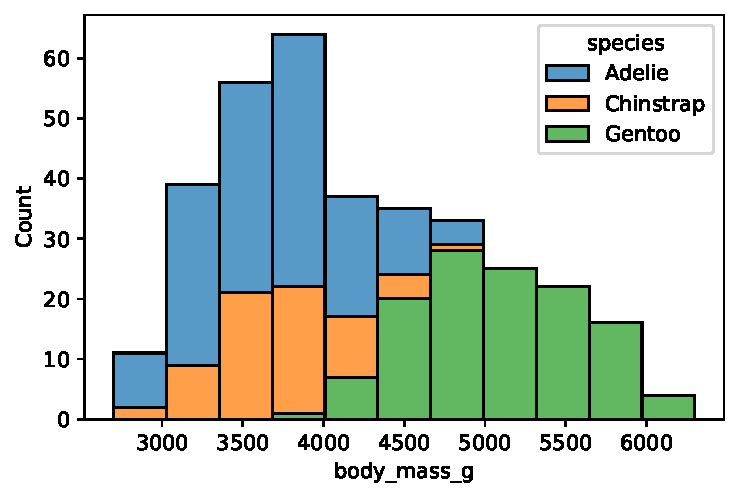
\includegraphics{chapters/numerical_by_categorical_files/figure-pdf/cell-4-output-1.pdf}

Observa que la forma del diagrama es la misma que la del histograma que
se realizó en la Sección~\ref{sec-1numerical-histogram}. La novedad es
que cada una de las barras que representa el número de pingüinos en cada
uno de los intervalos de peso se ha fragmentado en tres barras indicando
la contribución de cada especie. Aprecia que conforme va aumentando el
peso, va disminuyendo la contribución de las especies Adelie (azul) y
Chinstrap (naranja), y aumentando la contribución de la especie Gentoo
(verde).

Con el argumento \texttt{hue="species"} conseguimos que los datos se
dividan según las categorías de la variable \texttt{species} y se asigne
un color diferente a cada categoría, que se indica en la leyenda de la
esquina superior derecha del gráfico.

Y con el argumento \texttt{multiple="stack"} indicamos que las barras de
cada especie se dibujen apiladas en cada intervalo.

\begin{tcolorbox}[enhanced jigsaw, bottomrule=.15mm, colframe=quarto-callout-note-color-frame, toprule=.15mm, leftrule=.75mm, breakable, left=2mm, arc=.35mm, rightrule=.15mm, colback=white, opacityback=0]
\begin{minipage}[t]{5.5mm}
\textcolor{quarto-callout-note-color}{\faInfo}
\end{minipage}%
\begin{minipage}[t]{\textwidth - 5.5mm}

Para crear un histograma de barras apiladas de una variable numérica por
categorías, usa la función \texttt{histplot()} del paquete
\texttt{seaborn} conforme aprendiste en la sección
Sección~\ref{sec-1numerical-histogram} y además:

\begin{itemize}
\tightlist
\item
  indica el nombre de la variable que determina las categorías como
  valor del parámetro \texttt{hue}.
\item
  usa \texttt{multiple="stack"} para que las barras de las diferentes
  categorías se muestren apiladas.
\end{itemize}

\end{minipage}%
\end{tcolorbox}

\begin{exercise}[]% 
\protect\hypertarget{exr-histogram-stack}{}\label{exr-histogram-stack}%
Crea un histograma de barras apiladas para el peso de los pingüinos por
sexo.

\end{exercise}

\subsubsection{Histograma de barras
separadas}\label{histograma-de-barras-separadas}

Para crear un histograma del peso con barras separadas para cada especie
ejecuta la siguiente instrucción:

\begin{Shaded}
\begin{Highlighting}[]
\NormalTok{sns.histplot(}
\NormalTok{    data}\OperatorTok{=}\NormalTok{penguins,  }
\NormalTok{    x}\OperatorTok{=}\StringTok{"body\_mass\_g"}\NormalTok{, }
\NormalTok{    hue}\OperatorTok{=}\StringTok{"species"}\NormalTok{,}
\NormalTok{    multiple}\OperatorTok{=}\StringTok{"dodge"}
\NormalTok{)}\OperatorTok{;}
\end{Highlighting}
\end{Shaded}

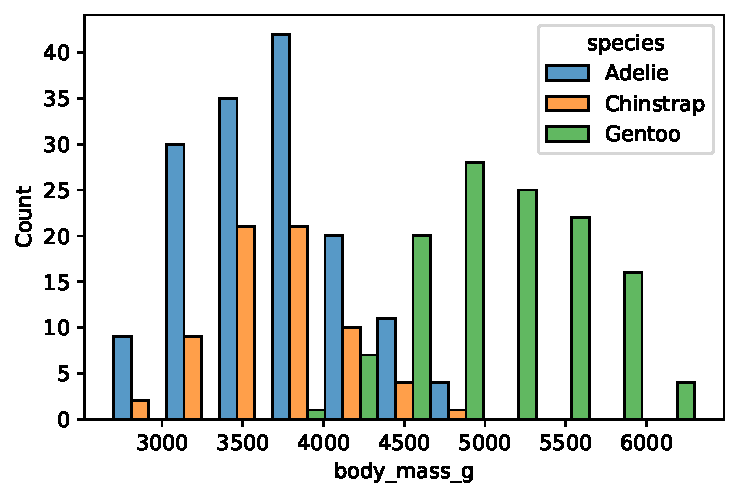
\includegraphics{chapters/numerical_by_categorical_files/figure-pdf/cell-5-output-1.pdf}

En este tipo de histograma fijándonos en las barras de un solo color
vemos el histograma de la especie correspondiente.

\begin{tcolorbox}[enhanced jigsaw, bottomrule=.15mm, colframe=quarto-callout-note-color-frame, toprule=.15mm, leftrule=.75mm, breakable, left=2mm, arc=.35mm, rightrule=.15mm, colback=white, opacityback=0]
\begin{minipage}[t]{5.5mm}
\textcolor{quarto-callout-note-color}{\faInfo}
\end{minipage}%
\begin{minipage}[t]{\textwidth - 5.5mm}

Para crear un histograma de barras separadas procede de la misma forma
que para crear un histograma de barras apiladas pero cambia el valor del
parámetro \texttt{multiple} a \texttt{"dodge"}.

\end{minipage}%
\end{tcolorbox}

\begin{exercise}[]% 
\protect\hypertarget{exr-histogram-stack}{}\label{exr-histogram-stack}%
Crea un histograma de barras separadas para la longitud del pico de los
pingüinos por sexo.

\end{exercise}

\subsubsection{Mosaico de histogramas}\label{mosaico-de-histogramas}

En los dos apartados anteriores aprendiste a crear dos tipos de
histogramas para visualizar la distribución de una variable numérica
distinguiendo varias categorías con colores diferentes en un mismo
gráfico. Pero a veces puede resultar más útil realizar histogramas
independientes para cada categoría. En este apartado aprenderás a crear,
de forma simultánea, tres histogramas con la distribución del peso de
los pingüinos de cada especie.

Con este fin el paquete \texttt{seaborn} proporciona la clase
\texttt{FacetGrid}, que permite crear un mosaico o una malla en la que
ubicar los diferentes gráficos para los datos de cada categoría.

Para entender cómo se usa la clase \texttt{FacetGrid} empieza ejecutando
la siguiente instrucción:

\begin{Shaded}
\begin{Highlighting}[]
\NormalTok{sns.FacetGrid(data}\OperatorTok{=}\NormalTok{penguins, col}\OperatorTok{=}\StringTok{"species"}\NormalTok{)}
\end{Highlighting}
\end{Shaded}

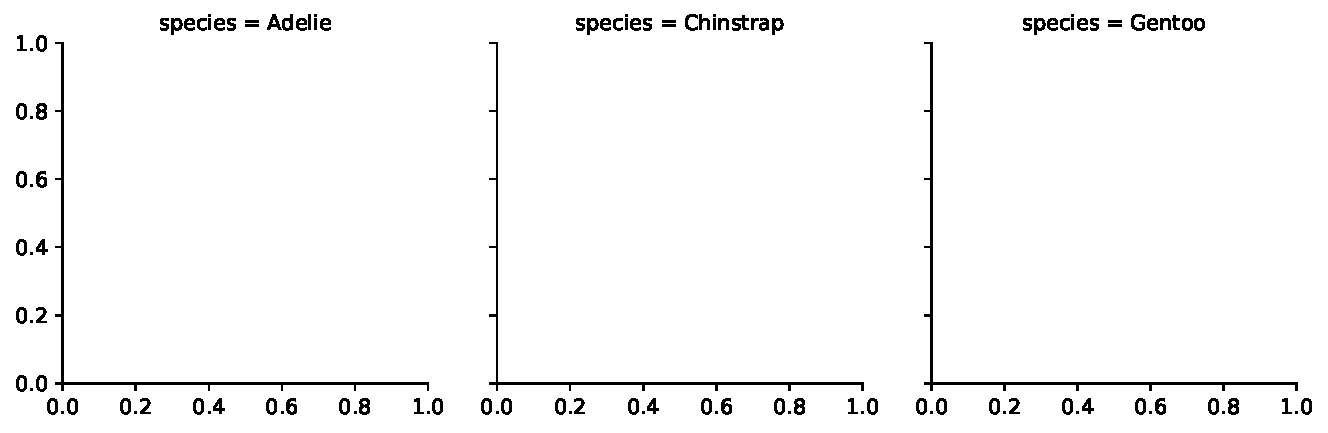
\includegraphics{chapters/numerical_by_categorical_files/figure-pdf/cell-6-output-1.pdf}

Observa el resultado y aprecia que se han creado tres ejes de
coordenadas, uno para cada especie. El efecto del argumento
\texttt{col="species"} es que se ha creado una columna
(\texttt{col}=\emph{column}) para cada categoría de la variable
\texttt{species}.

De momento hemos inicializado el mosaico pero aún no hemos dibujado nada
en cada una de las celdas del mosaico. Para hacerlo tenemos que aplicar
al mosaico el método \texttt{map()}, como en el siguiente ejemplo:

\begin{Shaded}
\begin{Highlighting}[]
\NormalTok{grid }\OperatorTok{=}\NormalTok{ sns.FacetGrid(data }\OperatorTok{=}\NormalTok{ penguins, col}\OperatorTok{=}\StringTok{"species"}\NormalTok{)}
\NormalTok{grid.}\BuiltInTok{map}\NormalTok{(sns.histplot, }\StringTok{"body\_mass\_g"}\NormalTok{)}\OperatorTok{;}
\end{Highlighting}
\end{Shaded}

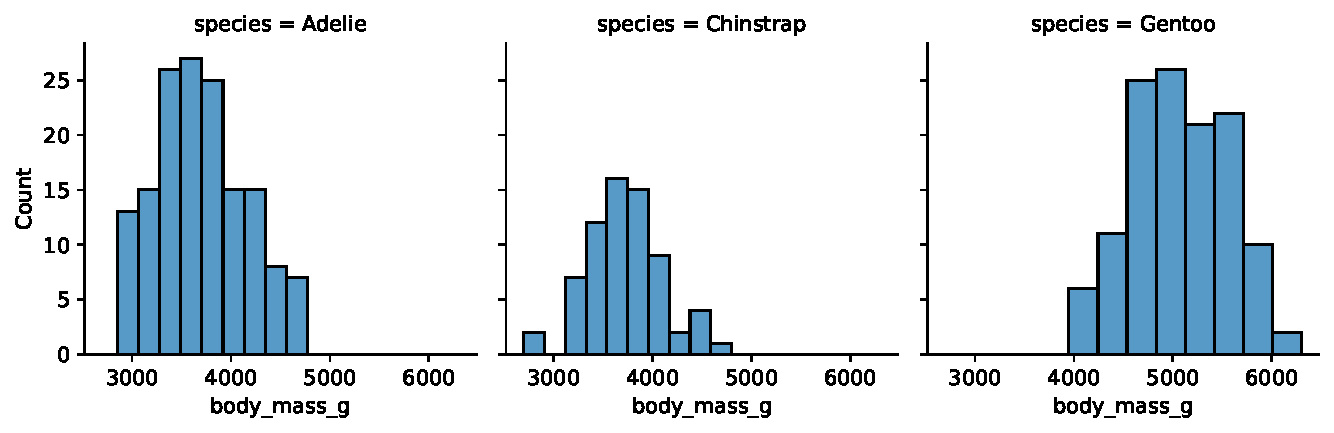
\includegraphics{chapters/numerical_by_categorical_files/figure-pdf/cell-7-output-1.pdf}

\begin{tcolorbox}[enhanced jigsaw, bottomrule=.15mm, colframe=quarto-callout-important-color-frame, toprule=.15mm, leftrule=.75mm, breakable, left=2mm, arc=.35mm, rightrule=.15mm, colback=white, opacityback=0]
\begin{minipage}[t]{5.5mm}
\textcolor{quarto-callout-important-color}{\faExclamation}
\end{minipage}%
\begin{minipage}[t]{\textwidth - 5.5mm}

Para que puedas visualizar el gráfico anterior en tu cuaderno de
\emph{Colab} tienes que escribir las dos instrucciones anteriores en la
misma celda.

\end{minipage}%
\end{tcolorbox}

Fíjate en las dos etapas que se han seguido en el ejemplo anterior para
la construcción de los tres histogramas:

\begin{enumerate}
\def\labelenumi{\arabic{enumi}.}
\item
  La primera instrucción

  \VERB|\NormalTok{grid }\OperatorTok{=}\NormalTok{ sns.FacetGrid(data }\OperatorTok{=}\NormalTok{ penguins, col}\OperatorTok{=}\StringTok{"species"}\NormalTok{)}|

  crea el mosaico con las tres columnas para las tres especies, y lo
  almacena en un nuevo objeto de nombre \texttt{grid} (puedes usar
  cualquier otro nombre).

  \begin{tcolorbox}[enhanced jigsaw, bottomrule=.15mm, colframe=quarto-callout-note-color-frame, toprule=.15mm, leftrule=.75mm, breakable, left=2mm, arc=.35mm, rightrule=.15mm, colback=white, opacityback=0]
  \begin{minipage}[t]{5.5mm}
  \textcolor{quarto-callout-note-color}{\faInfo}
  \end{minipage}%
  \begin{minipage}[t]{\textwidth - 5.5mm}

  Para inicializar un mosaico de gráficos con una columna para cada
  valor de una variable categórica, inicializa la clase
  \texttt{FacetGrid} indicando:

  \begin{itemize}
  \tightlist
  \item
    La hoja de datos como valor del parámetro \texttt{data}
  \item
    El nombre de la variable categórica para crear los grupos como valor
    del parámetro \texttt{col}
  \end{itemize}

  \end{minipage}%
  \end{tcolorbox}

  En este punto tenemos preparadas tres celdas para crear en cada celda
  un gráfico de los datos de la especie correspondiente a esa celda. La
  creación efectiva de los gráficos se realiza en el siguiente paso.
\item
  La segunda instrucción

  \VERB|\NormalTok{grid.}\BuiltInTok{map}\NormalTok{(sns.histplot, }\StringTok{"body\_mass\_g"}\NormalTok{)}|

  aplica el método \texttt{map()} al mosaico creado en el paso anterior,
  especificando qué tipo de gráfico queremos en cada celda del mosaico,
  y a qué variable queremos aplicar ese gráfico:

  \begin{itemize}
  \tightlist
  \item
    El primer argumento \texttt{sns.histplot} indica que en cada celda
    queremos realizar un histograma (para el grupo de datos de la
    especie correspondiente a la celda).
  \item
    El segundo argumento \texttt{"body\_mass\_g"} indica la variable de
    la que queremos hacer los histogramas.
  \end{itemize}

  \begin{tcolorbox}[enhanced jigsaw, bottomrule=.15mm, colframe=quarto-callout-note-color-frame, toprule=.15mm, leftrule=.75mm, breakable, left=2mm, arc=.35mm, rightrule=.15mm, colback=white, opacityback=0]
  \begin{minipage}[t]{5.5mm}
  \textcolor{quarto-callout-note-color}{\faInfo}
  \end{minipage}%
  \begin{minipage}[t]{\textwidth - 5.5mm}

  Para crear sendos gráficos de los datos asociados a cada celda de un
  mosaico creado con \texttt{FacetGrid} usa el método \texttt{map()} con
  los siguientes argumentos:

  \begin{itemize}
  \tightlist
  \item
    La función para construir los gráficos
  \item
    El nombre de la variable a la que aplicar esa función gráfica
  \end{itemize}

  \end{minipage}%
  \end{tcolorbox}
\end{enumerate}

\begin{exercise}[]% 
\protect\hypertarget{exr-facetgrid}{}\label{exr-facetgrid}%
Usa la clase \texttt{FacetGrid} para realizar sendos histogramas de la
distribución del peso para hembras y machos.

\end{exercise}

\begin{center}\rule{0.5\linewidth}{0.5pt}\end{center}

Si al inicializar la clase \texttt{FacetGrid} se usa el parámetro
\texttt{row} en lugar de \texttt{col} los diferentes gráficos aparecerán
dispuestos por filas en lugar de por columnas. Por ejemplo:

\begin{Shaded}
\begin{Highlighting}[]
\NormalTok{grid }\OperatorTok{=}\NormalTok{ sns.FacetGrid(data }\OperatorTok{=}\NormalTok{ penguins, row}\OperatorTok{=}\StringTok{"species"}\NormalTok{)}
\NormalTok{grid.}\BuiltInTok{map}\NormalTok{(sns.histplot, }\StringTok{"body\_mass\_g"}\NormalTok{)}\OperatorTok{;}
\end{Highlighting}
\end{Shaded}

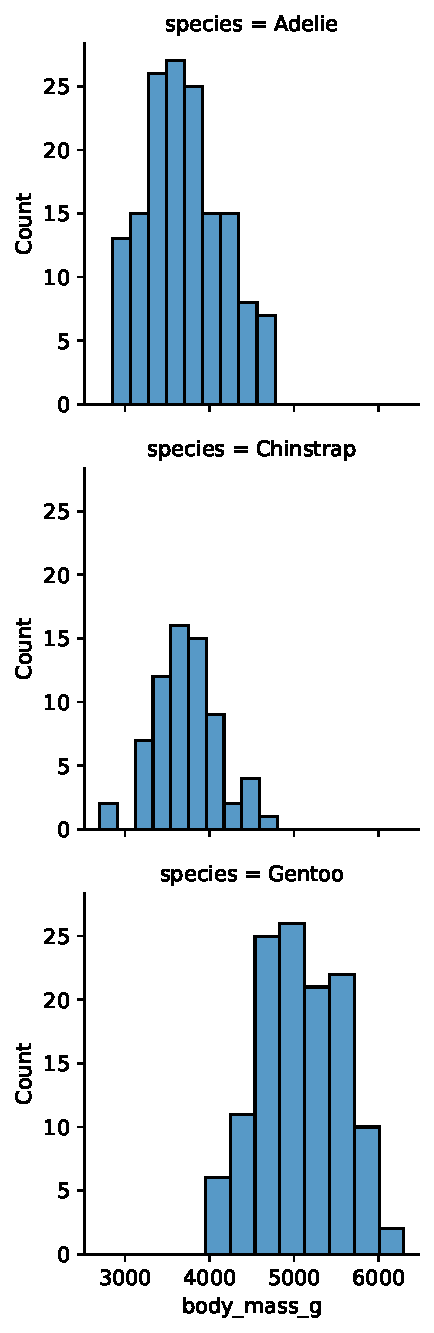
\includegraphics{chapters/numerical_by_categorical_files/figure-pdf/cell-9-output-1.pdf}

De hecho, se pueden usar los argumentos \texttt{row} y \texttt{col} al
mismo tiempo para crear un mosaico bidimensional. Las siguientes
instrucciones crean un mosaico de histogramas del peso de los pingüinos,
distinguiendo la especie por filas y el sexo por columnas, de
dimensiones \(3 \times 2\):

\begin{Shaded}
\begin{Highlighting}[]
\NormalTok{grid }\OperatorTok{=}\NormalTok{ sns.FacetGrid(data }\OperatorTok{=}\NormalTok{ penguins, row}\OperatorTok{=}\StringTok{"sex"}\NormalTok{, col}\OperatorTok{=}\StringTok{"species"}\NormalTok{)}
\NormalTok{grid.}\BuiltInTok{map}\NormalTok{(sns.histplot, }\StringTok{"body\_mass\_g"}\NormalTok{)}\OperatorTok{;}
\end{Highlighting}
\end{Shaded}

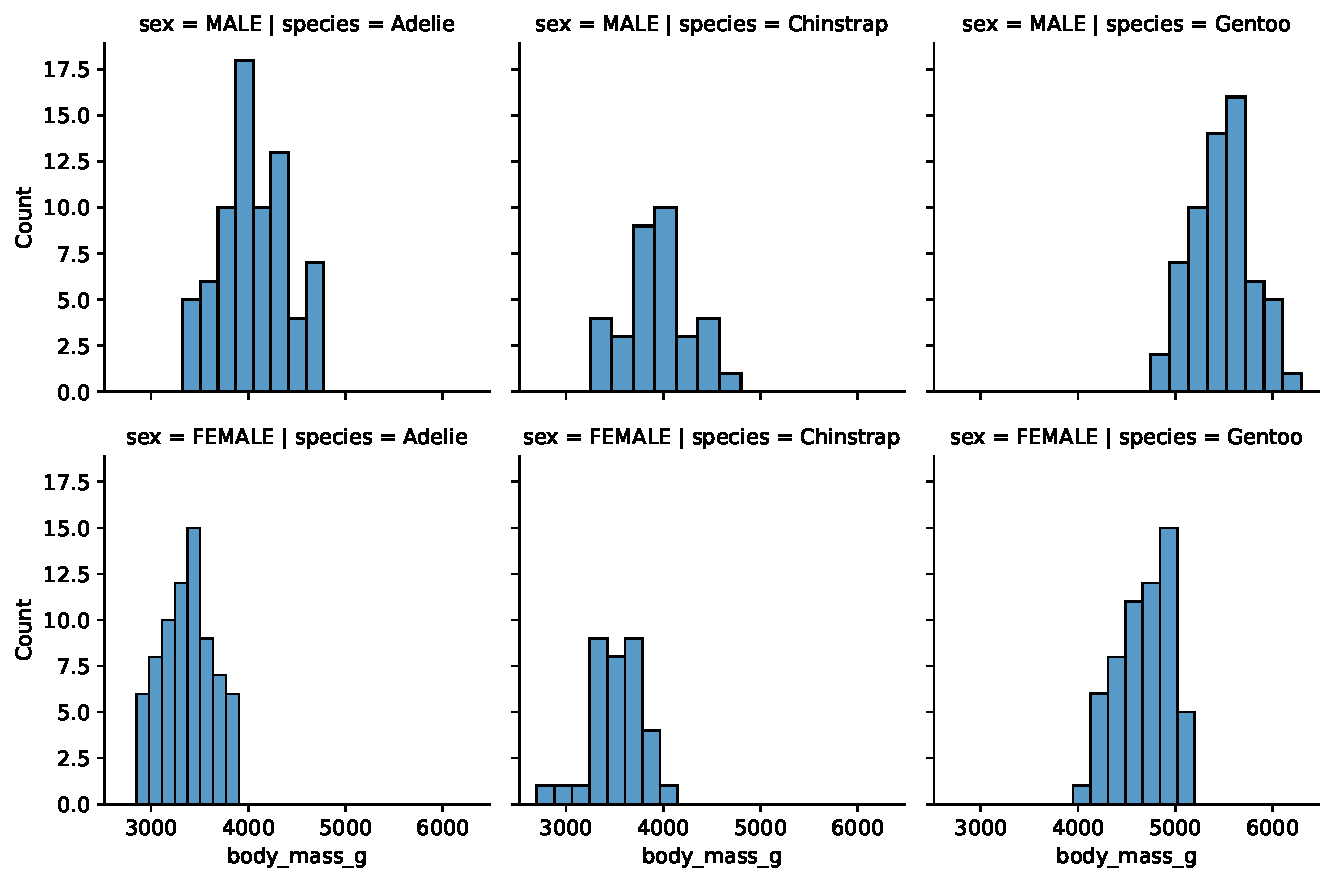
\includegraphics{chapters/numerical_by_categorical_files/figure-pdf/cell-10-output-1.pdf}

\begin{exercise}[]% 
\protect\hypertarget{exr-FacetGrid-3x2}{}\label{exr-FacetGrid-3x2}%
Usa \texttt{FacetGrid} para crear un mosaico de histogramas para la
longitud de las alas de los pingüinos distingüiendo la isla en la que
viven y su sexo.

\end{exercise}

\subsection{Diagramas de caja y
bigotes}\label{diagramas-de-caja-y-bigotes}

Para acabar la práctica realizaremos el gráfico de la portada de este
documento 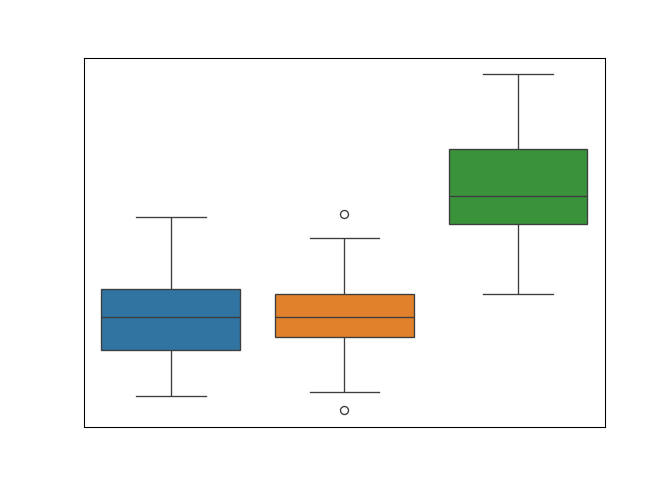
\includegraphics{chapters/../img/cover/cover.png}

en el que se representa un diagrama de caja y bigotes para el peso de
los pingüinos de cada especie.

En la Sección~\ref{sec-1numerical-boxplot} hicimos un diagrama de caja y
bigotes para el peso de todos los pingüinos (sin distinguir la especie)
con la instrucción

\begin{Shaded}
\begin{Highlighting}[]
\NormalTok{sns.boxplot(data}\OperatorTok{=}\NormalTok{penguins, y}\OperatorTok{=}\StringTok{"body\_mass\_g"}\NormalTok{)}\OperatorTok{;}
\end{Highlighting}
\end{Shaded}

Para diferenciar por especie no tenemos más que añadir el argumento
\texttt{x="species"}:

\begin{Shaded}
\begin{Highlighting}[]
\NormalTok{sns.boxplot(data}\OperatorTok{=}\NormalTok{penguins, x}\OperatorTok{=}\StringTok{"species"}\NormalTok{, y}\OperatorTok{=}\StringTok{"body\_mass\_g"}\NormalTok{)}\OperatorTok{;}
\end{Highlighting}
\end{Shaded}

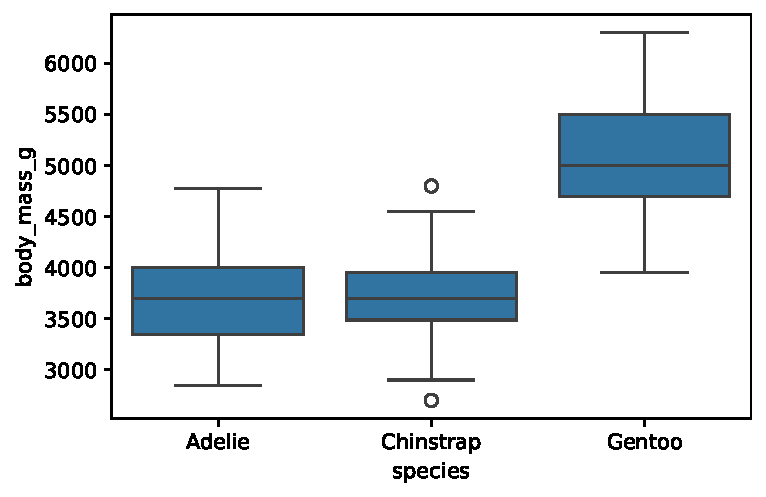
\includegraphics{chapters/numerical_by_categorical_files/figure-pdf/cell-12-output-1.pdf}

Para asignar un color diferente a cada especie añadimos
\texttt{hue="species"}:

\begin{Shaded}
\begin{Highlighting}[]
\NormalTok{sns.boxplot(data}\OperatorTok{=}\NormalTok{penguins, x}\OperatorTok{=}\StringTok{"species"}\NormalTok{, y}\OperatorTok{=}\StringTok{"body\_mass\_g"}\NormalTok{, hue}\OperatorTok{=}\StringTok{"species"}\NormalTok{)}\OperatorTok{;}
\end{Highlighting}
\end{Shaded}

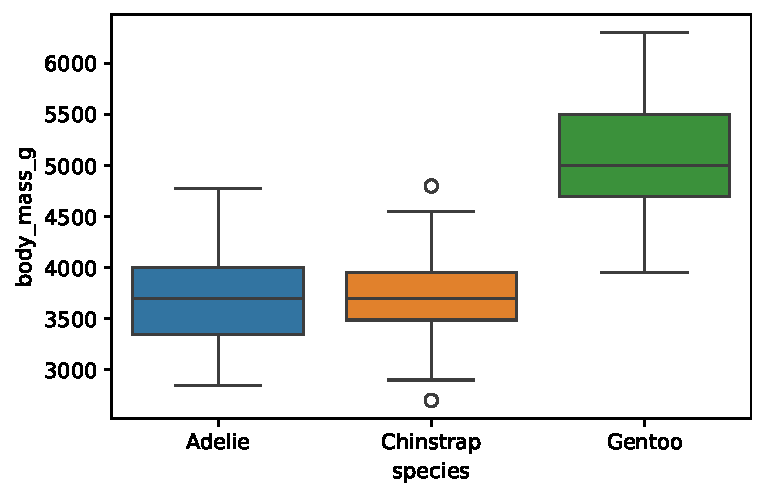
\includegraphics{chapters/numerical_by_categorical_files/figure-pdf/cell-13-output-1.pdf}

Los dos puntos que aparecen resaltados con un círculo fuera de los
bigotes en el diagrama de la especie Chinstrap (en naranja) son
\textbf{outliers}. El outlier por debajo del bigote inferior representa
un pingüino de la especie Chinstrap con peso excesivamente bajo, y el
outlier por encima del bigote superior se corresponde con un pingüino de
la especie Chinstrap con peso excesivamente alto (excesivamente
bajo/alto respecto a la distribución del peso en los pingüinos de la
especie Chinstrap).

\begin{exercise}[]% 
\protect\hypertarget{exr-boxplots}{}\label{exr-boxplots}%
Realiza un gráfico que muestre los diagramas de caja y bigotes para el
peso de las hembras y de los machos.

¿Aparecen outliers en alguno de los dos grupos?

\end{exercise}

\bookmarksetup{startatroot}



\cleardoublepage
\printsols
\myprintbibliography[title=Bibliografía]


\end{document}
